\documentclass[10pt,a4paper]{scrbook}
\usepackage[T1]{fontenc}
\usepackage[utf8]{inputenc}
\usepackage{ngerman,latexsym, longtable, amsmath, amssymb, latexsym,graphicx, enumitem, float, pstricks, stmaryrd, MnSymbol, array, linearb, titlesec}

%Mehr Raum zwischen subsections
\titlespacing{\section}{0pt}{*4}{*2.5}
\titlespacing{\subsection}{0pt}{*3.5}{*1.5}

% kleine Anpassungen, damit die Seitenbreite überall gleich ist.
\setcounter{secnumdepth}{2}
\setlength{\textwidth}{160mm}
\setlength{\textheight}{220mm}
\setlength{\headheight}{3mm}
\evensidemargin1mm
\oddsidemargin1mm

% Damit die Aufzählung wie in der Vorlesung ist.
\renewcommand{\thechapter}{\Roman{chapter}}
\renewcommand{\thesection}{\thechapter.\arabic{section}}
\renewcommand{\thesubsection}{\thesection.\arabic{subsection}}
\renewcommand{\thesubsubsection}{\thesubsection.\arabic{subsubsection}}

% Farbanpassung für die Graphen
\newrgbcolor{pgreen}{0 1 0}
\newrgbcolor{pblue}{0 0 1}
\newrgbcolor{pgrey}{0.6 0.6 0.6}


%Dokumentenanfang mit diversen input von mehreren Einzeldokumenten.
\begin{document}
	\begin{titlepage} 
\qquad\\
\vspace{4cm}

 	\begin{center} 
		{\Huge LAG+ Skript 
	\\[2ex] \small{basierend auf den Mitschriften von Maicon Hieronymus in \LaTeX \ gebracht von Sven Bamberger \par } }
		\vspace{2cm}
	 	\begin{figure} [H]
				\centering
				
\includegraphics[width=12cm, height=8cm]{front/pics/Logo.jpg}
		\end{figure}

	 	 Mainz,  \today 
	\end{center} 
 \end{titlepage}  
	
	\frontmatter 
		Dieses Skript wurde erstellt, um sich besser auf die Klausur vorzubereiten und eine ordentliche und für alle Personen lesbare Mitschrift zu haben. \\
\qquad\\
\qquad\\
\textcolor{red}{\Large{Dieses Dokument garantiert weder Richtigkeit noch Vollständigkeit, da es aus Mitschriften gefertigt wurde und dabei immer Fehler entstehen können. Falls ein Fehler enthalten ist, bitte melden oder selbst korrigieren und neu hochladen.}}
\qquad\\
\qquad\\
\large{Hier kleine Notizen zu einzelne Besonderheiten dieses Dokumentes.} \\
\normalsize{
\begin{enumerate}
	\item /* \qquad */  alles zwischen diesen Zeichen sind Kommentare und sollen zum tiferen Verständnis oder Besondere Fragestellungen darstellen. Dabei ist zu beachten, das die Notation nciht immer komplett korrekt ist.Es können also kleinere mathematische Fehler auftauchen, welche aber für das Verständnis relevant sind.
\end{enumerate}
}
		 
\tableofcontents 
 
	 
	\mainmatter 
		\chapter{Grundlagen} 
 	
	\section{Abbildungen}

\subsection{Idee:}
Es seien $A$ und $B$ Mengen. Unter einer Abbildung $f$ stellen wir uns einen Algorithmus vor, der aus jeder eingabe $a \in A$ ein eindeutig bestimmte Ausgabe $b \in B$ errechnet, $b$ ist nur durch $a$ (und $f$) festgelegt.

\begin{figure} [H]
\centering 
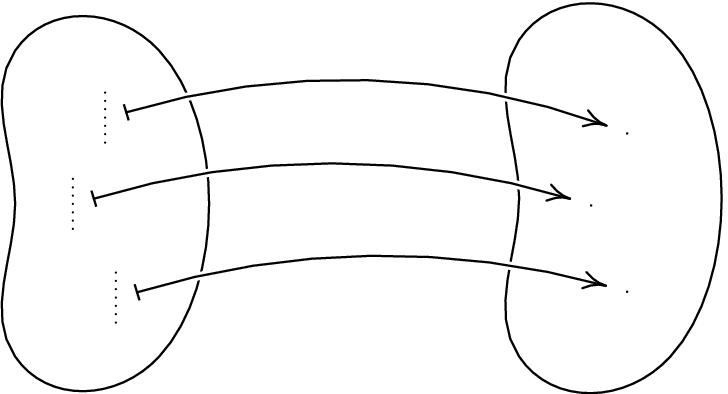
\includegraphics[width=10cm, height=6cm]{mainmatter/chapter1/pics/abbildunggenerell.png}
\caption{Eine einfache Abbildung} 
\end{figure}
%
%
%
\subsection{Definition:}

Es seien $A$ und $B$ Mengen. Eine Abbildung $f$ mit $ f:A \rightarrow B $ sei eine Teilmenge $f$ von $AxB = \{ (a,b) | a \in A, b \in B \}$ so, dass gilt:

\begin{description} 
\item[-] zu jedem $a \in A$ existiert ein $b \in B$ mit $(a,b) \ in f$ 
\item[-] sind $(a,b_{1}), (a,b_{2}) \in f$, so gilt $b_{1} = b_{2}$
\end{description}

$f$ ist also das, was in der Schule im Fall reller Funktionen als Graph der Funktion bezeichnet wurde. Anstatt $(a,b) \in f$ schreiben wir $b = f(a)$. Die Menge $A$ heißt Definitionsbereich von $f$, die Menge $B$ heißt Zielbereich von $f$. Ferner sei Bild $f = \{b \in B | \exists a \in A$ mit $f(a) = b\} = \{f(a) |  a \in A\} = f(A))$ (Wertebereich)
%
%
%
\subsection{Beispiel:}
	\begin{enumerate} 

		\item Vorzeichenfunktion $sign.$ $\mathbb{Z} \rightarrow\{-1,0,1\}$ $sign= \{(z,1)|z < 0\} \cup \{(0,0)\} \cup \{(z,1)|z > 0\}$

		\item  Identität: Für jede Menge $A$ sei $id_{A}: A \rightarrow A$ gegeben durch $id_{A} (b)=a$ $ \forall a \in A$

		\begin{description}
			\item[ ]{\pgreen $f:\mathbb{R}\rightarrow \mathbb{R}$, $f(a) = a^{2}$ $\forall a \in \mathbb{R}$}
			\item[ ]{\pblue $g:\mathbb{R}\rightarrow \mathbb{R}$, $g(a)=2a$ $\forall a\in \mathbb{R}$}
				\begin{figure} [H]
				\centering 
				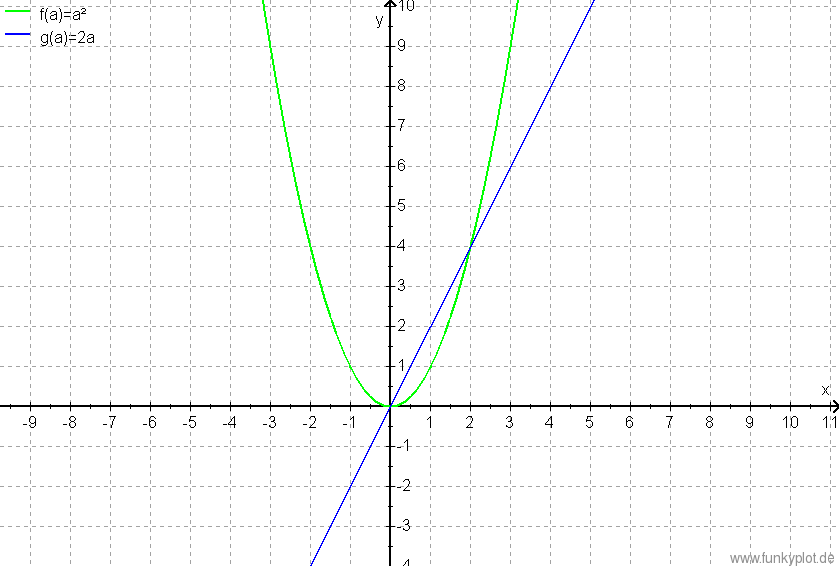
\includegraphics[width=14cm, height=8cm]{mainmatter/chapter1/pics/graph.png}
				\caption{Ein Beispiel Graph} 
				\end{figure}
			\item[ ] Bild $f=\{b \in \mathbb{R} | b \geq 0\} \subsetneqq \mathbb{R}$
			\item[ ] Bild $g = \mathbb{R}$
		\end{description}
		
		\item $g:\mathbb{Z}\rightarrow\mathbb{Z}$, $g(a)=\{2a|a\in\mathbb{Z}\} \subsetneqq \mathbb{Z}$ (Kurzschreibweise: $(=2\mathbb{Z})$)

	\end{enumerate} 
%
%
%
\subsection{Definition:}
Eine Abbildung $f: A \rightarrow B$ heiße:

	\begin{description}
		\item[-] surjektiv, falls Bild $f = B$ ist d.h., falls $\forall b \in B$ ein $a \in A$ existiert mit $f(a)=b$


		\item[-] injektiv, falls es zu jedem $b \in B$ höchstens ein $a \in A$ gibt mit $f(a)=b$.
		\begin{description}
			\item[] d.h.
			\item[-]  aus $f(a_{1}) = f(a_{2})$ folgt $a_{1}=a_{2}$
			\item[-] aus $a_{1} \neq a_{2}$ folgt $f(a_{1}) \neq f(a_{2})$
		\end{description}
		
		\item[-] bijektiv, falls $f$ injektiv und surjektiv ist 
				\begin{figure} [H]
				\centering 
				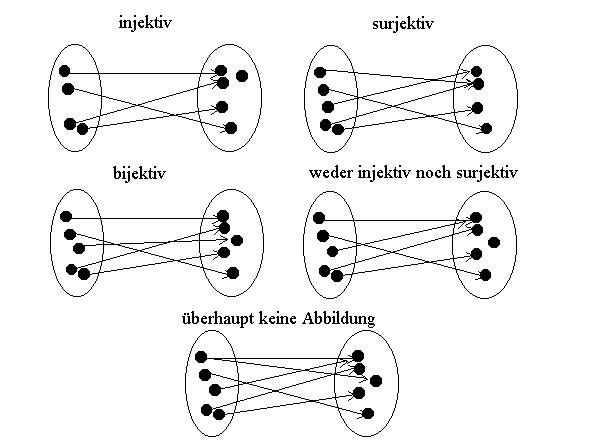
\includegraphics[width=17cm, height=10cm]{mainmatter/chapter1/pics/abbildungen.jpg}
				\caption{Mögliche Abbildungen auf einen Blick} 
				\end{figure}
	\end{description}


%
%
%
\subsection{Beispiel:}
	Sei $\mathbb{R}_{\geq0}=\{a \in \mathbb{R}|a \geq 0\}$
	\begin{enumerate}
		\item $f: \mathbb{R} \rightarrow \mathbb{R}$, $f(a)=a^{2}$ nicht surjektiv, nicht injektiv $(-1 \notin$ Bild $f)$ $((-1)^{2} = 1^{2})$
		\item $f: \mathbb{R} \rightarrow \mathbb{R}_{\geq0}$, $f(a) = a^{2}$ surjektiv, nicht injektiv
		\item $f: \mathbb{R}_{\geq0} \rightarrow \mathbb{R}$, $f(a) = a^{2}$ nicht surjektiv, injektiv
		\item $f: \mathbb{R}_{\geq0} \rightarrow \mathbb{R}_{\geq0}$, $f(a) = a^{2}$ bijektiv
	\end{enumerate}
%
%
%
\subsection{Definition}
\subsubsection{Komposition von Abbildungen }

Es seien $f: A \rightarrow B$ und $g: B\rightarrow C$ Abbildungen. 
Wir definieren $g \circ f: A\rightarrow C$ vermöge $(g \circ f) (a) = g(f(a))$ $\forall a\in A$
				\begin{figure} [H]
				\centering
				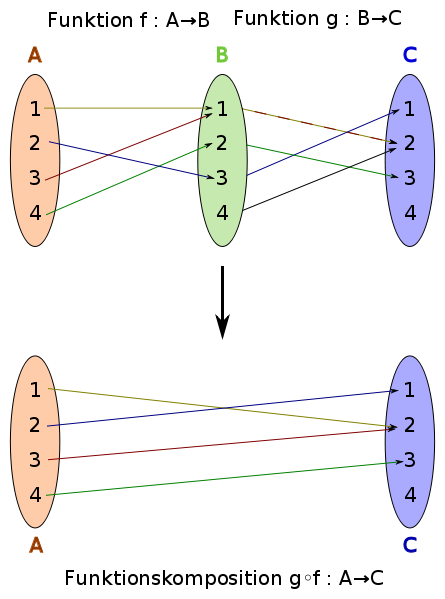
\includegraphics[width=6cm, height=8cm]{mainmatter/chapter1/pics/komposition.png}
				\caption{Eine mögliche Komposition} 
				\end{figure}
%
%
%
\subsection{Beispiel}
$f,g: \mathbb{R} \rightarrow \mathbb{R}$, $f(x)=x^{2}$, $g(x)=2x$ $\forall x \in \mathbb{R}$ 
	\begin{description}
		\item[] Dann:
		\begin{description}
			\item[] $(g \circ f)(x) = g(f(x)) = g(x^{2}) = 2x^{2}$
			\item[] $(f \circ g)(x) = f(g(x)) = f(2x) = (2x)^{2} = 4x^{2}$
		\end{description}
	\end{description}
Es kommt auf die Reihenfolge von f und g an!
%
%
%
\subsection{Satz}

Seien $f: A \rightarrow B$ und $g:B \rightarrow A$ Abbildungen mit $g \circ f = id_{A}$ Dann ist $f$ injektiv und $g$ surjektiv.

	\subsubsection{Beweis:}
		$f$ injektiv: Seien $a_{1},a_{2} \in A$ mit $ f(a_{1}) = f(a_{2}) $ z.z. $a_{1} = a_{2}$
		\begin{description}
			\item[]  Dazu: $a_{1} = id_{A}(a_{1}) = (g \circ f) (a_{1}) = g(f(1_{1})) = g(f(a_{2})) = (g \circ f)(a_{2}) = id_{A} (a_{2}) = a_{2}$
			\item[] g surjektiv: Sei $a \in A$ (=Zielbereich von g)
			\item[] z.z. Es gibt ein $b \in B$ (=Definitionsbereich von g) mit $g(f(a)) = (g \circ f)(a) = id_{A}(a) = a$ wähle daher $b=f(a)$
		\end{description}
	/* $f: A \rightarrow B$\qquad $ f\circ id_{A}:A\rightarrow B$\qquad $f\circ id_{A}=f$ */

\subsection{Definition:}
	In der Situation I.1.8 nennen wir $g$ eine linksinverse von $f$ und $f$ eine rechtsinverse von $g$.

\subsection{Definition:}
	Ist $f: A \rightarrow B$ bijektiv, so sei die zu $f$ inverse Abbildung $f^{-1}: B \rightarrow A$ gegeben durch $f^{-1} = \{ (b,a) \in B$x$A| a,b \in f\}$

		\begin{description}
			\item[Warnung:] Das klappt nur bei bijektiven Abbildungen $f$, da $f_{-1}$ beidseitig invers zu $f$ ist. 
			\item[Hinweis:] $f^{-1}$ inverse der Abbildung \qquad $f1^{-}$ volles Urbild jedoch ist dies nicht zwangsläufig bijektiv
		\end{description}

\subsection{Definition:}
	Sei $f:A \rightarrow B$ und $Y \leq B$. Dann nennen wir $j(Y) = \{ a \in A | f(a) \in Y\}$ das volle Urbild zu $Y$ unter $f$. 

		\begin{figure} [H]
		\centering 
		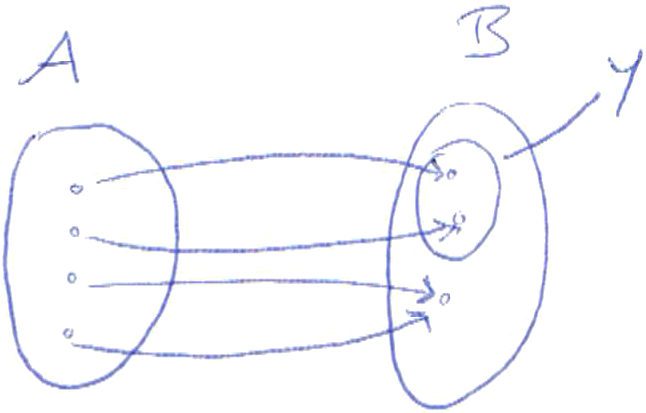
\includegraphics[width=5cm, height=3cm]{mainmatter/chapter1/pics/untermengen1.png}
		\caption{Eine Abbildung auf Untermengen} 
		\end{figure}
\subsection{Beispiel:}
In 1.5(1) war $f: \mathbb{R} \rightarrow \mathbb{R}$, $f(a)=a^{2}$.
$f(\{0,1,4\}) = \{-2,-1,0,1,2\}$

\begin{description}

	\item[Beispiel:] $g:\mathbb{Z} \rightarrow \mathbb{Z}$, $g(a)=a^{2}$ \\
	$f^{-}(\{0,1,2,3,4\}) = \{-2,-1,0,1,2\}$

\end{description}

	\section{Äquivalenzrelationen}

\subsection{Bemerkung:}
	Es sei $f: A \rightarrow B$ eine Abbildung. Für jedes feste $b \in B$ nennen wir $f^{-}(b) = \{ a \in A | f(a) = b\}$ die Faster von $b$ unter $f$. Offenbar sind je zwei Fasern disjunkt: $b_{1} \neq b_{2} \Longrightarrow f^{-} (b_{1}) \cap j(b_{2}) = \emptyset$ ferner ist $ A =  	\mathop{\bigcup}\limits_{b \in B} j(b)$. Wir sprechen von einer disjunkten Zerlegung bzw. Partition von $A$. /*  Faser $\mathrel{\widehat{=}}$ volles Urbild; disjunkt = Schnitt ist leer. */ 

\subsection{Beispiel:}
	$ A =$ Menge aller Autos. \\
	$ F =$ Menge aller Farbcodes von Autos.\\
	$f: A \rightarrow F$ ordnet jedem Auto seinen Farbcode zu. Damit werde die Autos andhand ihrer Farbe ( Faser von blaue ( blaue Autos)) in unterschiedliche Schubladen gepackt, die Faser von $f$. Die Fasern sind disjunkt, da jedes Auto einen bestimmten Farbcode hat. Jedes Auto hat einen Farbcode, liegt also in einer Faser. \\
Vermöge $f$ können zwei Autos gleicher Farbe als "`gleichwertig"' angesehen werden. 

\subsection{Definition:}
Eine Äquivalenzrelation auf einer Menge $A$ sei eine Teilmenge von $!_{R}$ von $A$x$A$ mit folgenden Eigenschaften:
\begin{description}

	\item[R ist refelxiv:] für jedes $a \in A$ ist $(a,a) \in $ R
	\item[R ist symmetrisch:] ist $(a_{1}, a_{2}) \in $ R, so auch $(a_{2},a_{1}) \in$ R
	\item[R ist transitiv:] sind $(a_{1}, a_{2}),(a_{2}, a_{3}) \in$ R, so auch $(a_{1},a_{3}) \in$ R

\end{description}
Anstatt $(a,b) \in$ R schreiben wir $a \sim_{R} b$ und sagen "`a äquivalent b"'.

\subsection{Beispiel:}

  \begin{enumerate}[label={\alph*)}]
     \item zu Beispiel 2.2 ist $\mathbb{R} = \{ (a,b) \in A$x$A|f(a) = f(b)\}$ eine Äquivalenzrelation auf der Menge $A$ aller Autos. 
     \item Auf jede Menge ist die Gleichheit "`="' von Elmenten eine Äquivalenzrelation. 
	\item Kongruenz von Dreiecken in der Zeichenebene $R^{2}$ ist eine Äquivalenzrelation auf der Menge dieser Dreiecke.
  \end{enumerate} 
%
%
%
\subsubsection{Erinnerung}
	Äquivalenzrelation $\sim$ auf $M$
\begin{description}
	\item [-] reflexiv $\forall a \in M a \sim a$
	\item [-] symmetrisch wenn $ a \sim b$, dann $b \sim a$
	\item [-] transitiv wenn $a \sim b \wedge b \sim c$, dann $a \sim c$
\end{description}
%
%
%
\subsection{Definition:}

Es sei $\sim$ eine Äquivalenzrelation auf $M$. Für jede \\
$a \in M$ sei $\{ b \in M | a \sim b\} = [a] =_{wegen Symmetrie} \{b \in M | b\sim a\}$ die sogenannte \underline{Äquivalenzklasse} zu a. \\
Jedes $b \in [a]$ heiße ein \underline{Vertreter} von $[a]$. 
\begin{description}
	\item[\underline{Beachte:}] Reflexivität $\Rightarrow a$ Vertreter von $[a]$ (wegen Symmetrie).
\end{description}
%
%
%
\subsection{Hauptsatz:}
Es sei $M$ eine feste Menge. Dann gilt:
\begin{description}
	\item[-] Die Äquivalenzrelationen auf $M$ entsprechen genau den Partitionen von $M$.
\end{description}
Genauer:
\begin{description}
	\item[(a)] Ist $M = \mathop{\dot{\bigcup}}\limits_{i \in I}$ $M_{i}$ ($\dot{\bigcup}$  = disjunkte Vereinigung) eine Partition von $M$, so ist eine Äquivalenzrelation $\sim$ auf $M$ gegeben durch: $a \sim b \Leftrightarrow$ es gibt ein $i \in I$ mit $a,b \in M_{i}$ Die Äquivalenzklassen zu $\sim$ sind genau die Mengen $M_{i} (i \in I)$
	\item[(b)] Ist $\sim$ eine Äquivalenzrelation auf $M$, so bilden die 'quivalenzklassen zu $\sim$ eine Partition von M.
	\item[(c)] Die durch $(a)$ und $(b)$ gegebenen Abbildungen sind bijektiv und gegenseitig invers. 
		\begin{figure} [H]
		\centering 
		
\includegraphics[width=8cm, height=5cm]{mainmatter/chapter1/pics/bijektivinvers.png}
		\caption{Eine bijektive und inverse Abbildung} 
		\end{figure}
\end{description}
%
%
%
\subsubsection{Beweis:}
\begin{description}
	\item[(a)] \quad
	\begin{description}
		\item[\underline{reflexiv:}] Sei $a \in M$. Dann existiert ein $i \in I$ mit $a \in M_{i} \Rightarrow a \sim a$.
		\item[\underline{symmetrisch:}] Seien $a,b \in M$ mit $a \sim b \Rightarrow \exists i \in I: a,b \in M_{i} \Rightarrow b \sim a$.
		\item[\underline{transitiv:}] Seien $a,b,c \in M$ mit $a \sim b$ und $b \sim c \Rightarrow$ es gibt $i \in I$ mit 
			$a,b \in M_{i}$ und es gibt $j\in J$ mit $b,c \in M_{j}$ Da $b \in M_{i} \wedge M_{j}$ und die Partition $M 
			= \mathop{\dot{\bigcup}}\limits_{i \in I} M_{i}$ disjunkt ist, ist $i = j \Rightarrow a,c \in M_{i} = M_{j}$ und somit $a \sim 
			c$. Nach Definition von $\sim$ ist $[a] = M_{i}$ für das einzige $i \in I$ mit $a \in M_{i}$
	\end{description}
	\item[(b)] Jeder $a \in M$ liegt in einer Äquivalenzklasse, z.B. in $[a]$. Also genügt es z.z.: Verschiedene 	
		Äquivalenzklassen zu $\sim$ sind sogar disjunkt. Seien dazu $a,b \in M$ mit $[a] \cap [b] \neq \emptyset$ 
		\underline{zeige} $[a] = [b]$. \\
		Wähle $c \in [a] \cap [b]$. Dann: $a \sim c$ und $c \sim b$ transitiv $\Rightarrow a \sim b \Rightarrow a \in [b]$ 
		und $b \in [a]$. \\
		Ist nun $x \in [a]$, so $x \sim a$ und $a \sim b$, somit $x \sim b$ und $x \in [b]$. \\ 
		Fazit: $[a] \subseteq [b]$ \ \ Analog: $[b] \subseteq [a]$
	\item[(c)] Die Abbildungen sind offentsichtlich zueinander invers, daher bijektiv.
\end{description}
%
%
%
\subsection{Bemerkung:}
Gemäß 2.1 liefern die nicht leeren Fasern einer Abbildung $f: A \rightarrow B$ eine Partition von $A$, also eine Äquivalenzrelation auf $A$.\\
Umgekehrt kann zu jeder Partition $A =  \mathop{\dot{\bigcup}}\limits_{i \in I} A_{i}$ von $A$ eine Abbildung $g: A \rightarrow I$ definiert werden via $g(a) = i$ falls $a \in A_{i}$\\
Dann $A_{i} = g(i)$ und die Partition der $A_{i}$ ist die Faser-Partition von g.













		\chapter{Elementare Zahlentheorie}

	\section{Teilbarkeit}

\subsection{Definition:}
Seien $a,b \in \mathbb{Z}$. Gibt es ein $s \in \mathbb{Z}$ mit $a = b\cdot s$, so sagen wir "`b teilt a"', schreiben $b|a$ und nennen $b$ einen \underline{Teiler} von a. 
%
%
%
\subsection{Bemerkung:}
\begin{description}
	\item[-] aus $a|b$ und $a|c$ folgt stets $a|(b\pm c)$ \\
		$(b=a\cdot x)$ und $c =a\cdot y \Rightarrow b\pm c = a(x\pm y))$

	\item[-] aus $a|b$ und $c|d$ folgt stets $ac|bd$ \\
		$(b=ax)$ und $d =c\cdot y \Rightarrow bd = (ac)(xy)$
\end{description}
%
%
%
\subsection{Satz:}
Sei $n \in \mathbb{N}_{\diagdown\{0\}}$ \underline{fest}. eine Äquivalenzrelation $\equiv_{n}$ auf $\mathbb{Z}$ ist gegeben durch: $ a \equiv_{n} b \Leftrightarrow n|(b-a)$ (sogenannte Kongruenz modulo n)
%
%
%
\subsection{Beweis:}
\begin{description}
	\item[- \underline{reflexiv:}] Sei $ a \in \mathbb{Z}$. Da $ 0 = n\cdot  0$, ist $n \diagdown 0 = (a-b)$\\
						 $\Rightarrow a \equiv_{n} 
					  a$
	\item[- \underline{symmetrisch:}] Seien $a,b \in \mathbb{Z}$ mit $a \equiv_{n} b \Rightarrow n|(b-a)$\\
						$\Rightarrow n|(a-b) \Rightarrow bn\equiv_{n} a$
	
	\item[- \underline{transitiv:}] Seien $a,b \in \mathbb{Z}$ mit $a\equiv_{n} b$ und $b\equiv_{n} c$ \\
						$\Rightarrow n|(b-a)$ und $n|(c-b)$ \\
						$\Rightarrow^{\small{1.2}} n|(c-b) + (b-a) = c-a$\\
						$\Rightarrow a \equiv_{n} c$
\end{description}
%
%
%
\subsection{Satz:} 
Die Äquivalenzklasse zu $\equiv_{n}$ sind genau: $[0], [1], [2], \dotsc  , [n-1]$ Insbesondere gilt die sogenannte \underline{Division mit Rest} in $\mathbb{Z}$: zu gegebenen $a \in \mathbb{Z}, 0 < n \in \mathbb{N}$ existieren $q, r \in \mathbb{Z}$ mit $ a= qn+r$ und $r \in \{0,\dotsc  , n-1\}$ und $q$ und $r$ sind \underline{eindeutig} bestimmt.

\begin{description}
	\item[\underline{Beweis:}] Sei $K$ eine Äquivalenzklasse zu $\equiv_{n}$. Wähle $r \in \mathbb{N}$ minimal bzgl. $r \in 
					K$. 
	\begin{description}
		\item[Beachte:] $K$ enthält eine natürliche Zahl. Ist $ a\in K$ negativ, so addiere ein Vielfaches $q\cdot n$ von $n$ 
					sodass $a+qn > 0$. Dann ist $n|qn=(a+qn)-a$, also $a+qn \in K$. \\
					Dann ist $r \in \{0,\dotsc  , n-q\}$, dann wäre $r \geq n$, so $n|n=r-(r-n)$ also $r-n\in K$ 
					 natürliche Zahl $< r$. $\lightning$\\
					Somit ist $K$ eine der Äquivalenzklassen $[0], [1], \dotsc  , [n-1]$\\
					Sei nun $0 \leq r < s \leq n-1$
		\item[Annahme:] $[r] = [s] \Rightarrow r\equiv_{n} s, n| s-r \quad \lightning$ zu $0 < s-r < n$
		\item[Fazit:] $[r] \neq [s]$ \\
				Damit $\mathbb{Z} = [0]$ $\dot{\bigcup}$ $[1]$ $\dot{\bigcup} \dotsc   $ $\dot{\bigcup}$ $[n-1]$ \\
				Ist $ a \in \mathbb{Z}$, so $a \in [r]$ für ein $r \in \{ 0, \dotsc  , n-1\} \Rightarrow n|a-r$ \\
				also: $a-r=qn$ für ein $q \in \mathbb{Z}, a =qn+r$
	\end{description}
	\item[Eindeutigkeit von q und r:] \qquad\\
						Sei $q_{1}n+r_{1}=a=q_{2}n+r_{2}$ mit $r_{1}, r_{2} \in \{0, \dotsc  , n-1\}$ \\
						Dann: ($q_{1}-q_{2})n=r_{2}-r_{1}$, $n|r_{2}-r_{1}$, $r_{1}\equiv_{n} r_{2} 
						\Rightarrow r$.\\
						Somit $(q_{1} -a_{2}) \cdot n = 0 \Rightarrow^{n\neq 0} q_{1}-a_{2} = 0$, $q_{1} 
						= q_{2} \qquad \square$\\
\end{description}
%
%
%
\subsection{Definition:} Eine natürliche Zahl $p \geq 2$ heißt Primzahl, wenn $1$ und $p$ die einzigigen natürlichen Zahlen 
				sind, die p teilen.
\begin{description}
	\item[Also:] $2, 3, 5, 7, 11, 13, 17, 19, 23, 29, 31, \dotsc  $
\end{description}
%
%
%
\subsubsection{Satz:}

\begin{enumerate}[label={\alph*)}]
     \item Jede natürliche Zahl $n \geq 2$ ist ein Produkt von Primzahlen.
     \item Euklid: Es gibt unendlich viele Primzahlen
\end{enumerate}
\begin{description}
	\item[Beweis:] \quad \\
		\begin{enumerate}[label={\alph*)}]
			\item Wähle einen kleinsten Teiler $> 1$ von $n$. Dieser muß Primzhal sein, also $n=p \cdot b$ mit $b < 
				n$. Zerlege nun $b$ weiter.
			\item \underline{Annahme} $p_{1}, \dotsc  , p_{s}$ sind die einzigen Primzahlen. 
			\begin{description}
				\item[Bild:] $m=p_{1}, \dotsc  , p_{s}+1$. Nach $(a)$ muss einer der $p_{i}$ Teiler von m 
					      sein.
				\item[Dann:] $p_{i}|m$ und $p_{i}|p_{1}-p_{s} \Rightarrow ^{1.2} p_{i}| m-p_{1}-p_{2} = 1 
						\quad \lightning$
			\end{description}
		\end{enumerate}
\end{description}
%
%
%
\subsection{Fundamentalsatz der Zahlentheorie} 
$0 \neq z \in \mathbb{Z}$ Dann hat $z$ eine \underline{eindeutige} Darstellung der Form $z = \varepsilon \cdot p_{1} \cdot p_{2} \cdot \dotsc   \cdot p_{s}$ mit $\varepsilon \in \{\pm1 \}, p_{1}\leq p_{2} \leq \dotsc   \leq p_{s}$ Primzahlen.
	\begin{description}
		\item[Beweis:] o.E. $z \geq 0$ Induktion nach $z$. $z = 1$ Wähle $s = 0$
		\begin{description}
			\item[] \underline{$Z \geq z$} Sei $z =p_{1}, \dotsc , p_{z} = q_{1}, \dotsc , q_{t}$ für gewisse 
				Primzahlen $p_{i}, q_{j}$ mit $p_{1} \leq \dotsc   \leq p_{s}, q_{1} \leq \dotsc   \leq q_{t}$.
			\item[] \underline{z.z.:} $s=t$ und $p_{i} = a_{i}$ für $1 \leq i \leq s$.\\
				$s \geq$ und $ t\geq 1$\\
				o.E. $p_{1} \leq q_{1}$
			\item[] Annahme: $p_{1} \lneqq q_{1} \leq q_{2} \leq \dotsc \leq q_{t}$ \\
				Division mit Rest durch $p_{1}$ \qquad $q_{j} = a_{j} p_{1} + rj$ mit $0 \leq rj < p_{1}$ Da 
				$p_{j}$ Primzahl $\Rightarrow rj > 0 für 1 \leq j \leq t$.
			\item[] Betrachte: $m=r_{1}, r_{2} \dotsc r_{t} < p^{t}_{1} < q_{1} \cdot q_{2} \dotsc q_{t} = z$
			\item[] Induktion $\Rightarrow m$ hat \underline{eindeutige} Zerlegung im Produkt vin Primzahlen 
				 Insbesondere $p_{1}\ndivides m$ (da $p_{1}\ndivides rj \quad \forall j$) \\
				Nun: $m = (q_{1} -a_{1}p_{1})(q_{2}-a_{2}p_{1})\dotsc (q_{t}-a_{t}p_{1}) = q_{1} \cdot q_{2} 
				\dotsc q_{t} + p_{1} (\dotsc) \Rightarrow^{p_{4}|2} p_{1}|m \ \lightning$
			\item[] Fazit: $p_{1} = q_{q}$ und $p_{2} \dotsc p_{s} = q_{2} \dotsc q_{t}$\\
					Induktion liefer $p_{j} = q_{j}$ für $z \leq j \leq t =s$
		\end{description}
	\end{description}
%
%
%
\subsection{Definition:} Für $a,b \in \mathbb{Z}\diagdown\{0\}$ sei
	\begin{description}
	\item[] 
		\begin{description}
		\item[]
		\item[-] $ggT(a,b) = max \{d\in \mathbb{Z} \ | \ d|a \wedge d|b\}$
		\item[-] \underline{kleinster gemeinsamer Vielfaches} $kgV(a,b) = min\{c\in\mathbb{N} \ | \ a|c\wedge b|c\}$
		\end{description}
	\end{description}
%
%
%
\subsection{Bemerkung:}
Ist $a = \pm p^{\alpha_{1}}_{1} \dotsc p^{\alpha_{s}}_{s}$ und $b = \pm p^{\beta_{1}}_{1} \dotsc p^{\beta_{s}}_{s}$ mit Primzahlen $p_{1} < p_{2} < \dotsc p_{s}$ und gewissen $\alpha_{i} \geq 0, \ \beta_{i} \geq 0$, so gilt $ggT(a,b) = p^{\gamma_{1}}_{1} \dotsc p^{\gamma_{s}}_{s}$ wo $\gamma = min\{\alpha_{i}\beta_{i}\}$\\
$kgV(a,b) = p^{\delta_{1}}_{1} \dotsc p^{\delta_{s}}_{s}$ wo $\delta_{i} = max\{ \alpha_{i}, \beta_{i}\}$\\
Insbesondere: $\gamma_{i} + \delta_{i} = \alpha_{i} + \beta_{i}$ und daher $|a\cdot b| = ggT(a,b) \cdot kgV(a,b)$
%
%
%
\subsection{\underline{Euklidischer Algorithmus}}
Zur Bestimmung von $ggT(a,b)$\\
Seien $a,b \in \mathbb{Z} \diagdown\{0\}$
	\begin{enumerate}
		\item Setze $a_{0} = |a|$, $a_{1} = |b|$, o.E. $q_{1} < q_{0}$
		\item Wiederhole Division mit Rest:\\
			$q_{i-1} = q_{i} \cdot a_{i} + a_{i+1}$ wo $0 \leq a_{i+1} <a_{i}$
		\item Ergibt sich erstmalig $a_{m+1} = 0$, so ist $a_{m} = ggT(a,b)$\\
			Beispiel:
		\begin{description}
			\item[] $a=90, b=84$
			\item[] $90 = a = 1\cdot 84+6$
			\item[] $84 = 14 \cdot 6 +0$
			\item $\Rightarrow 6 = ggT(90,84)$
		\end{description}
	\end{enumerate}
%
%
%
\subsection{ } /* Fehlerhafte Nummerierung an der Tafel, oder in der Mitschrift. */
%
%
%
\subsection{Satz} Der Euklidischer Alogorithmus terminiert und liefert den $ggT$ 
\begin{description}
	\item[Beweis:] Er terminiert, da $a_{0} > a_{1} > a_{2} > \dotsc > a_{m} > a_{m+1} \geq 0$ in $\mathbb{N}$
	\item[Zwischenschritte:] 
	\begin{description}
		\item[-] Ist $a = q \cdot b+r$, so $ggT(a,b) = ggT(b,r)$
		\item[-] Ist $d|a$ und $d|b$, so $d|a-q\cdot b = r \Rightarrow d|b$ und $d|r$
		\item[-] Ist $d|b$ und $d|r$, so $d|q\cdot b + r = a \Rightarrow d|a$ und $d|b$
	\end{description}
\end{description}
Daher ergibt sich in 1.10\\
 $ggT(a,b) = ggT(a_{0}, q_{1}) = ggT(a_{1}, q_{2}) = ggT(a_{2}, q_{3}) = ggT(a_{m-1}, q_{m}) \equiv a_{m}$\\
/* $0 = a_{am+1}$, d.h. $a_{m-1}=q_{m} \cdot a_{m+0} =$ dem oben genannten $\equiv$ */
%
%
%
\subsection{Bemerkung:}
Der Euklidische Algorithmus ist schnell.
%
%
%
\subsection{Erweiterter Euklidischer Algorithmus}
Mit der Notation aus 1.10 berechnen wir zustäzlich für $0 \leq j \leq m$ ganze Zahlen $v_{i},v_{j}$ wie folgt:
\begin{description}
	\item[-] in Schritt 1$u_{0} = 1, v_{0}=0, u_{1}=0, v_{1}=1$
	\item[-] in jedem Durchlauf der Schleife 2: \\
			$u_{i+1} = v_{i-1} - q_{i} \cdot u_{i}$\\
			$v_{i+1} = v_{i-1} - q_{i} \cdot v_{i}$
\end{description}
Dann gilt $\forall i$: $a_{i} = u_{i} \cdot a_{0} + v_{i} \cdot a_{i}$ \\
Insbesondere ist am Ende $a_{m} = u_{m} \cdot a_{0} + v_{m} \cdot a_{1} = ggT (a_{0}, q_{1})$
	\begin{description}
		\item[\underline{Beweis:}]
		\begin{description}
			\item[] mit Induktion nach $i$:
			\item[\underline{$i = 0$}] $a_{0} = 1 \cdot a_{0} + 0 \cdot a_{1}\  \checkmark $
			\item[\underline{$i = 1$}] $a_{1} = 0 \cdot a_1{0} + 1 \cdot a_{1} \ \checkmark $
			\item[\underline{$1\leq i \rightarrow i + 1$}] $a_{i-1} = a_{i-1} - q_{i} \cdot a_{i} =^{Ind}(u_{i-1} \cdot 
						a_{0} + v_{i-1} \cdot a_{1}) - q_{i}(u_{i} \cdot a_{0} + v_{i} \cdot a_{1})$
			\item[\qquad] \ \ \qquad $ = a_{0} \underbrace{(u_{i-1}-q_{i} \cdot u_{i})} + a_{1}\underbrace{(v_{i-1} 
						- q_{i}\cdot v_{i})}$
			\item[\qquad] \ \ \qquad \qquad \qquad $= u_{i}$ \qquad \qquad \qquad $= v_{i+1} \qquad \qquad 
						\square$
		\end{description}
	\end{description}
%
%
%
\subsection{Folgerung:}
Zu beliebigen $a,b \in \mathbb{Z} \diagdown\{0\}$ existieren $\underbrace{u,v \in \mathbb{Z}}$ mit $ggT(a,b) = u \cdot a+ v \cdot b$\\
.  \qquad \qquad \qquad \qquad \qquad \ sogenannte Bezout-Koeffizienten
%
%
%
\subsection{Beispiel:} 
$a_{0} = 245, \ a_{1} = 112$ \\
\begin{center}
	\begin{tabular} {cccc}
		$a_{i}$ & $q_{i}$ & $u_{i}$ & $v_{i}$ \\ \hline
		$245$   & \qquad  &    $1$    &     $0$ \\ 
		$112$   &  $2$      &	    $0$    &     $1$ \\
		$21$     &  $5$      &    $1$    &     $-2$ \\
		$7$       &  $3$      &    $-5$   &     $11$ \\
		$0$       &              &              &               \\
	\end{tabular} 
\end{center}
\qquad\\
\\
$7 = ggT(a_{0},a_{1}) = (-5) \cdot 245 + 11 \cdot 112$
	\section{Modulo Rechnen}
%
%
%
\subsection{Motivation}
Für ein festes $0 < n \in \mathbb{N}$ betrachten wir die Äquivalenzklassen zwischen Äquivalenzrelation $\equiv_{n}$. Es sei $\mathbb{Z}/n\mathbb{Z} = \{ [0], [1], \dotsc, [n-1]\}$. Wir wollen eine Addition und Multiplikation auf $\mathbb{Z}/n\mathbb{Z}$ einführen, so wie wir das von der Uhr (für $n=12$) gewöhnt sind. \\
$[a]+[b]=[a+b]$ und $[a] \cdot [b] = [a \cdot b] \forall \ a,b \in \mathbb{Z}$\\
Frage: Ist das möglich oder ergeben sich Widersprüche?
%
%
%
\subsection{Satz}
Die in 2.1 definierte Addition $ \ + \ \mathbb{Z}/n\mathbb{Z}$ x $\mathbb{Z}/n\mathbb{Z} \rightarrow \mathbb{Z}/n\mathbb{Z}$\\
und Multiplikation $ \ \cdot \ \mathbb{Z}/n\mathbb{Z}$ x $\mathbb{Z}/n\mathbb{Z} \rightarrow \mathbb{Z}/n\mathbb{Z}$ sind \underline{wohldefiniert} (widerspruchsfrei definiert), da das Ergebnis $[a] + [b]$ bzw. $[a] \cdot [b]$ nur von den Äquivalenzklassen $[a]$ und $[b]$ abhängt sind nicht von $a$ und $b$ selbst. 
\begin{description}
	\item[Beweis:] Seien $[a_{1}]  = [a_{2}], [b_{1}] = [b_{2}]$. Dann: $n|a_{2} - a_{1} \wedge n|b_{0} - b_{1}$\\
			$\Rightarrow n| a_{2} - a_{1} + b_{2} - b_{1} = (a_{2} + b_{2}) - (a_{1} + b_{1})$\\
			\quad \\
			$ \Rightarrow \underbrace{[a_{2}]+[b_{2}]} = \underbrace{[a_{1}+b_{1}]}$\\
			$. \quad [a_{2}] + [b_{2}] \quad [a_{1}] + [b_{2}]$
	\item[Ebenso:] $n| a_{2}(b_{2} - b_{2}) + b_{1}(a_{2} - a_{1}) = a_{2}b_{2} - a_{1}b_{1}$\\
				\quad\\
				$\Rightarrow \underbrace{[a_{2}b_{2}]} = \quad \underbrace{[a_{1}b_{1}]}$\\
				$. \quad [a_{2}][b_{2}] \quad [a_{1}][b_{1}]$
\end{description}
%
%
%
\subsection{Beispiel:} In $ \mathbb{Z}/12\mathbb{Z}$ gilt: $[11]^{2} = [11^{2}] = [121] = [1]$\\
				geschickter: $[11]^{2} = [-1]^{2} = [(-1)^{2}] = [1]$
\begin{description}
	\item[Beachte:] $[3] \cdot [4] = [3\cdot4] = [12] = [0]$ wobei $[3]$ und $[4]$ alleine gesehen jeweils $\neq 0$
\end{description}
Wenn klar ist, dass wir $\mathbb{Z}/n\mathbb{Z}$ rechnen für ein konstantes n, so lassen wir die Klammern i.d.R. weg.
%
%
%
\subsubsection{WDH:} $\mathbb{Z}/n\mathbb{Z} = \{ [0], [1], \dotsc, [n-1]\}$ \ $a \equiv_{n} \Leftrightarrow n|b-a$ für $a,b \in \mathbb{Z}$\\
$[a] + [b] = [a+b]$\\
$[a] \cdot [b] = [a \cdot b]$
%
%
%
\subsection{Bemerkung:}
Da $ + $ und $ \cdot $ in $\mathbb{Z}/n\mathbb{Z}$  auf die entsprechenden Rechenoperationen in $\mathbb{Z}$ zurückgeführt werden, erbt $\mathbb{Z}/n\mathbb{Z}$ die aus $\mathbb{Z}$ bekannten Rechengesetze.\\
\underline{Beachte jedoch:} Es kann elemente $x \neq u \neq y$ in $\mathbb{Z}/n\mathbb{Z}$ geben mit $x \cdot y = 0$. (etwa $[2] \cdot [3] = [0]$ in $\mathbb{Z}/6\mathbb{Z}$)\\
Solche $x,y$ heißen \underline{Nullteiler}. 
%
%
%
\subsection{Definition:} 
Wir nennen $x \in \mathbb{Z}/n\mathbb{Z}$ invertierbar, falls es in $y \in \mathbb{Z}/n\mathbb{Z}$ gibt mit $x \cdot y = 1$. Mit $(\mathbb{Z}/n\mathbb{Z})^{x}$ bezeichnen die Menge aller invertierbaren Elemente in $\mathbb{Z}/n\mathbb{Z}$. 
%
%
%
\subsection{Satz:}
$n \geq 1$ ist \underline{fest}. Für $a \in \mathbb{Z}$ sind äquivalent:
\begin{enumerate}
	\item $[a]$ ist invertierbar in $\mathbb{Z}/n\mathbb{Z}$
	\item $ggT(a,n) =1$
	\begin{description}
		\item[Beweis:] \qquad\\
		\begin{description}
			\item[$(1) \Rightarrow (2)$:] Sei $[a] \cdot [b] = [1]$, \qquad $n|ab - 1, n\cdot v = ab - 1$ für ein $v \in 
								\mathbb{Z}$\\
								.\quad $\Rightarrow 1 = ab - nv$\\
								.\quad Ist $q$ ein Teiler von $a$ und $n$, so auch von $1$. \\
								.\quad $\Rightarrow q = \pm 1, ggT(a,n) = 1$
			\item[$(1) \Rightarrow (2)$:] Sei $1 = ggT(a,n) = a \cdot u + n \cdot v$ für gewisse $u,v \in 
								\mathbb{Z}$\\
								.\quad $\Rightarrow n|nv = 1-au \Rightarrow [1] = [a]\cdot[a] \qquad 
									\square$
		\end{description}
	\end{description}
\end{enumerate}
%
%
%
\subsection{Folgerung:}
$(\mathbb{Z}/n\mathbb{Z})^{x}$ = $\{[a] | 0 < a < n$ und $ggT(a,n) = 1\}$. Ist $n=p$ eine Primzahl, so ist \underline{jedes} Element $\neq 0$ in $\mathbb{Z}/p\mathbb{Z}$ invertierbar.
\begin{description}
	\item[\underline{Beachte:}] \qquad
	\item[] Für $n=a\cdot b$ mit $0 < a \leq b < n$ wird dies falsch.
	\item[] $[a] \cdot [b] = [n] = [0]$
	\item[] Wäre nun $[c] \cdot [a] = [1]$, so $ [c] \cdot [a] \cdot [b] = [1] \cdot [b] = [b]$ wobei $[c] \cdot [0] = [0]$
\end{description}
%
%
%
\subsection{Definition:} 
$\varphi(n) = |(\mathbb{Z}/n\mathbb{Z})^{x}| = $ Anzahl der $ a \in \{ 1, \dotsc, n-1\}$ mit $ggT(a,n) = 1$.\\
Das definiert die \underline{eulersche $\varphi$ - Funktion} $\varphi : \mathbb{N}\diagdown\{0\} \rightarrow \mathbb{N}$
%
%
%
\subsection{Satz: (Euler)} 
\begin{description}
	\item[$n \geq 1$ \underline{fest}]. für jedes $x \in (\mathbb{Z}/n\mathbb{Z})^{x}$ gilt $x^{\varphi(n)} = 1$ \\ 
	\item[Mit anderen Worten:] Für jedes zu n teilerfremde $a\in \mathbb{Z}$ gilt $a^{\varphi(n)} \equiv_{n} 1$.\\
	\item[Insbesondere:] Ist $n = p$ Primzahl, so $x^{p} = x$ \ $\forall x \in \mathbb{Z}/n\mathbb{Z}$. (da $\varphi (p) 
					= p-1$)
\end{description}

\subsubsection{Beweis:}
Sei $(\mathbb{Z}/n\mathbb{Z})^{x} = \{x_{1}, x_{2}, \dotsc, x_{\varphi(n)}\}$\\
Für festes $ z\in (\mathbb{Z}/n\mathbb{Z})^{x}$ definieren wir $\alpha_{z} : (\mathbb{Z}/n\mathbb{Z})^{x} \rightarrow (\mathbb{Z}/n\mathbb{Z})^{x}$ durch $\alpha_{z} (x) = x \cdot z$ \ $\forall x \in (\mathbb{Z}/n\mathbb{Z})^{x}$\\
(da: $x \cdot z \cdot z^{-1} \cdot x^{-1} = x \cdot 1 \cdot x^{-1} = 1 \Rightarrow x z \in (\mathbb{Z}/n\mathbb{Z})^{x}$) Da z invertierbar ist $z \cdot y = 1 y \cdot z$ für ein $y \in (\mathbb{Z}/n\mathbb{Z})^{x}$ somit $\alpha_{z} \cdot  \alpha_{y} = id = \alpha_{y} \cdot \alpha_{z} \Rightarrow \alpha_{z}$ bijekktiv.\\
$\Rightarrow \alpha_{z}$ vertauscht die Elmente $x_{1}, x_{2}, \dotsc, x_{\varphi(n)}$\\
\qquad\\
Somit: $ \underbrace{\prod \limits^{\varphi(n)}_{i = 1} x_{i}} = \prod \limits^{\varphi(n)}_{i = 1} \alpha_{2} (x_{i}) = \prod \limits^{\varphi(n)}_{i = 1} (x_{i} \cdot z) = \underbrace{(\prod \limits^{\varphi(n)}_{i = 1} x_{i})}\cdot z^{\varphi(n)}$\\
.\ \quad \qquad $ =: d$ \qquad \qquad \qquad \qquad  \qquad \qquad \ \quad $= d$\\
\qquad\\
Multiplikation mit $d^{-1}$ liefert $1 = z^{\varphi(n)} \qquad \square$

	\section{Kryptographie}
%
%
%
\subsection{Ziel:}
Anna und Bruno wollen vertrauliche Nachrichten austauschen. Jedoch ist der Übertragungsweg unsicher. Sie wissen, dass der böse Lasko lauschen wird. Gibt es eine sichere Verschlüsselungsmethode?
%
%
%
\subsection{Problem:}
Alle klassischen Verfahren (z.B. Caesar-Verschlüsselung) arbeiten mit einem geheimen Schlüsselwort, welches von Anna und Bruno zuvor vereinbart werden muss. Insbesondere bei häufigem Wechsel des Schlüsselworts ist das schwierig, da persönliche Treffen in aller Regel zu aufwendig sind. 
%
%
%
\subsection{Erinnerung:}
Sei $0 < a \in \mathbb{R}$ fest. Die \underline{Logarithmusfunktion} $\log_{a}: ]0, \infty [ \rightarrow \mathbb{R}$ zu Basis $a$. ist die Inverse der Abbildung $a^{\BNccc}: \mathbb{R} \rightarrow ]0, \infty [$ speziell $a = e$ \ $x \rightarrow a^{x}$ für alle $ x \in \mathbb{R}$ liefert $ a^{\BNccc} = exp (\BNccc)$ \ $a^{x} = y \leftrightarrow x = \log_{a} y$ \\

\begin{figure} [H]
	\centering
	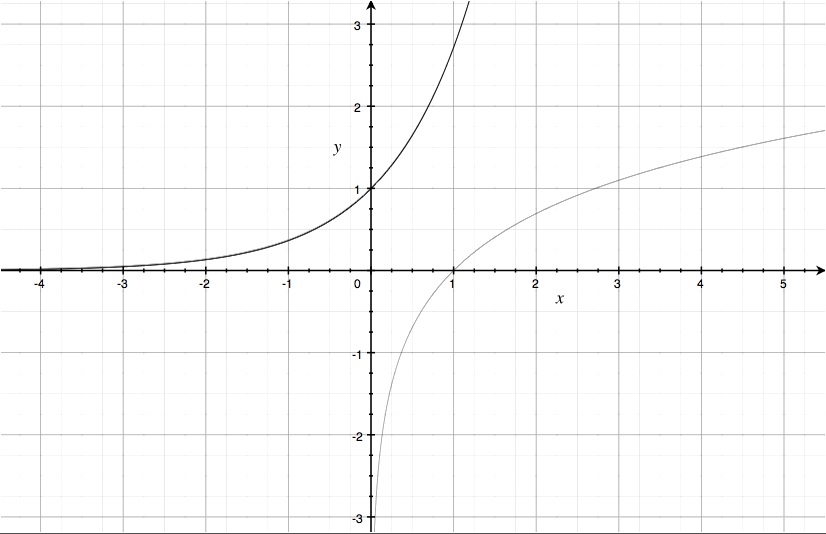
\includegraphics[width=12cm, height=8cm]{mainmatter/chapter2/pics/graphkryp.png}
	\caption{Es wurden $y_{1}= e^{x}$ und \pgrey{$y_{2}=\ln x$}} 
\end{figure}
%
%
%
\subsection{Definition:}
Es seien $ 2 \leq n \in \mathbb{N}$ und $0< a < n$ \underline{fest} gewählt. Gilt $a^{k} \equiv_{n} b$, so nennen wir $k$ einen \underline{diskreten Logarithmus} von $b$ zur Basis $a$ modulo $n$. 
%
%
%
\subsection{Beispiel:}
$n = 13$ \ $a = 7$\\
\qquad\\
\begin{tabular}{c|cccccccccccc} 
$b$ & 1 & 2 & 3 & 4 & 5 & 6 & 7 & 8 & 9 & 10 & 11 & 12 \\\hline 
$\log_{a} b$ mod $n$ & 12 & 11 & 8 & 10 & 3 & 7 & 1 & 9 & 4 & 2 & 5 & 6\\
\end{tabular} 
%
%
%
\subsection{Idee:}
\begin{description}
	\item[-] Die Abbildung $k \rightarrow a^{k}$ mod $n$ ist relativ rasch zu berechnen (vgl. 3.7).
	\item[-] Die Umkehrfunktion, des diskreten Logarithmus erlaubt mit heutigen Methoden keine systematische rasche Berechnung. 
\end{description}
Wir nennen daher $k \rightarrow a^{k} $ mod $ n$ eine Einwegsfunktion.
%
%
%
\subsection{Rasche Berechnung von  $\mathbf{a^{k}}$ mod $\mathbf{n}$}
Sei $k = \varepsilon_{0} \cdot 2^{0} + \varepsilon_{1} \cdot 2^{1} + \dotsc + \varepsilon_{s} \cdot 2^{s}$ mit $\varepsilon_{i} \in \{0,1\} = \sum \limits^{s}_{j = 0} \varepsilon_{j}2^{j}$ die eindeutige Binärdarstellung von  $k$.\\
Dann gilt:
\begin{equation*}
a^{k} = a^{\sum \limits^{s}_{j = 0} \varepsilon_{j}2^{j}} = \prod \limits^{s}_{j = 0} a^{\varepsilon_j s^{j}} = \prod \limits^{s}_{j=0}(a^{2^{j}})^{\varepsilon_j} = \prod \limits^{s}_{\varepsilon_{j = 1}} a^{2^{j}}
\end{equation*}
Wir berechnendaher die $a^{2^{j}}$ mod $n$ durch sukzessives Quadrieren und sofortiges Reduzieren modulo $n$.\\
\qquad\\
\underline{Beispiel:}\\
Berechne $3^{48}$ mod $23$: Dazu: $48 = 32 +16 = 2^{5} + 2^{4} = (110000)_{2}$
\begin{equation*}
	\begin{tabular}{c|c|c|c|c|c|c} 
		$j$ & $0$ & $1$ & $2$ & $3$ & $4$ & $5$ \\\hline 
		$3^{2^{j}}$ \ mod$_{23}$ & $3$ & $9$ & $81\equiv 12$ & $144 \equiv 6$ & $36  \equiv 13$ & $169 \equiv 9$\\
	\end{tabular} 
\end{equation*}
\underline{Fazit:}\\
Anstelle von $48$ Multiplikationen genügen $6$ Multiplikationen. \\
Schlüsseltauschalgorithmus ( Diffie-Hellmann)
\begin{description}
	\item[-] Anna \& Bruno vereinbaren öffentlich eine Primzahl $p$ und eine Basis $a \in \{2,\dotsc, p-2\}$
	\item[-] Anna \& Bruno wählen jeder für sich eine persönliche Geheimzahl $k_{A}$ bzw. $k_{B}$. 
	\item[-] Beide berechnen insgeheim $a^{k_{A}}$ mod $p = b_{A}$ bzw. $a^{k_{B}}$ mod $p=b_{B}$
	\item[-] Anna sendet $b_{A}$ an Bruno, Bruno sendet $b_{B}$ an Anna (öffentlich)
	\item[-] Nun können beide für sich den Rest $a^{k_{A}k_{B}}$ mod $p$ berechnen. 
\end{description}
Da\\
$a^{k_{A}k_{B}} = (a^{k_{B}})^{k_{B}} \equiv_{p} b_{A}^{k_{B}} \leftarrow$ Bruno!\\
$(a^{k_{B}})^{k_{A}} \equiv_{p} b_{B}^{k_{A}} \leftarrow$ Anna!\\
Damit haben beide die Geheimzahl $a^{k_{A}k_{B}}$ mod$p$ vereinbart
\begin{description}
	\item[-] Carlo kennt das ganze System, er kennt $a,p,b_{A},b_{B}$ und kann trotzdem nicht $a^{k_{A}k_{B}}$ mod$p$ berechnen.
\end{description}
%
%
%
\subsection{Definition:}
Es sei T eine Menge an Teilnehmern in einem Netzwerk.\\
Ein \underline{System öffentlicher Schlüssel} sei eine Familie $\{f_{t},g_{t}|t\in T\}$ von Abbildungen derart, dass gilt:
\begin{description}
	\item[-] $f_{t}$ ist eine öffentlich bekannte Einwegsfunktion
	\item[-] $g_{t}$ ist eine nur dem Teilnehmer $t$ bekannte Inverse zu $f_{t}$
\end{description}
%
%
%
\subsection{Definition:}
$T =$ Menge der Teilnehmer $ \{f_{t}, g_{t}|t \in T\}$ wo $f_{t}$ Einwegsfunktion mit Inverser $g_{t}$\\
 \underline{ System öffentlicher Schlüssel}
%
%
%
\subsection{Vorteile:}
\begin{description}
	\item[-] Gibt es ein solches System, in dem jeder Teilnehmer seinen Schlüssel $f_{t}, g_{t}$ selbst bestimmen kann, so entfällt der Schlüsseltausch.
	\item[-] Neue Teilnehmer können jederzeit hinzustoßen.
	\item[-] Spontane Kommunikation wird möglich
	\item[-] $n$ Teilnehmer benötigen lediglich $2\cdot n$Schlüssel. (anstelle $\frac{n(n-1)}{2}$ Schlüssel für Paare von Teilnehmern
\end{description}
%
%
%
\subsection{RSA-Verfahren}
\begin{enumerate}
	\item Schlüsselerzeugung
	\begin{description}
		\item[-] Teilnemer $t$ wählt zwei froße PRimzahlen $p_{t} \neq q_{t}$ und bildet $n_{t} = p_{t} \cdot q_{t}$. 					Dann berechnet $t$ die Eulersche $\varphi$ - Funktion $\varphi (n_{t})$\\
				Dies ist ganz einfach:\\
				Die einzigen Teiler $d \in \{1, \dotsc, n_{t-1}\}$ mit $ggT(d,n) \neq 1$ von $n_{t}$ zwischen $1$ 					und $n_{t}-1$ sind von der Form $p_{t} \cdot a$ (a geeignet ( $1 \leq a \leq q_{t} - 1$ )) oder 					$q_{t} \cdot b$ (b geeignet ( $1 \leq b \leq p_{t} - 1$))\\
				$\Rightarrow$ Es gibt genau ($q_{t} - 1$) + ($p_{t} - 1$) solche $d$.\\
				$\Rightarrow \varphi(n_{t}) = |\{ c | 0 <  c < n_{t},$ $ggT(c_{t},n_{t}) = 1\}| = (n_{t} - 1) - 					(q_{t} - 1) - (p_{t} - 1) = (p_{t} - 1)(q_{t} - 1)$
		\item[-] Nun wählt $t$ eine Zahl $k_{t} \in \{2, \dotsc, \varphi(n_{t}) -1\}$ teilerfram zu $\varphi(n_{t})$ (z.B. 					eine Primzahl $> \varphi(n_{t})$ reduziert modulo$\varphi(n_{t})$)
		\item[-] Mit dem erwarteten Euklid- Algorithmus bestimmt $t$ Zahlen $l_{t}$ und $v_{t}$ so dass $1 = k_{t} 					\cdot l_{t} + \varphi(n_{t}) \cdot v_{t}$
		\item[-] $t$ vernichtet vorraussichtlich $p_{t}, q_{t}, \varphi(n_{t}), v_{t}$ 
		\item[-] als öffentlichen Schlüssel gibt $t$ das Paar $(k_{t},n_{t})$ heraus $i$ als Geheimschlüssel verbleibt $l_{t}$ bei $t$. 
	\end{description}
	\item Die Sicherheit des Verfahrens beruht darauf, dass es für große $p_{t}, q_{t}$ keinen raschen, systematischen 			Weg gibt, um aus $n_{t}$ heraus $p_{t}, q_{t}$ oder $\varphi(n_{t})$ zu bestimmen.
	\item Kryptographie mittels RSA\\
		Anna will Bruno eine nachricht senden. Der Klartext sei eine große ganze Zahl. $x \in \{2, \dotsc, n_{B}-2\}$ (alle 
		ASCII-Zeichen einer Nachricht können in einer einzigen großen Zahl zusammengefasst werden.
	\begin{description}
		\item[-] Anna verschatt sicht den öffentlichen Schlüssel ($k_{b},n_{b}$) von Bruno
		\item[-] Bruno berechnet $z \equiv y^{l_{B}}$ mod$n_{B}$
		\item[-] Nach Satz von Euler (2.9) gilt: \\
				$z \equiv y^{l_{B}} \equiv x^{k_{B}l_{B} + v_{t} \varphi(n_{B})} \equiv x^{1} \equiv$ 						mod$n_{B}$
		\item[-] Es ist extrem unwahrscheinlich dass $ggT(x,n_{B}) \neq 1$ ist, da Anna sonst eine Zerlegung von 						$n_{B}$ gefunden hätte.
		\item[-] Carlo ist machtlos, da er aus $y, k_{B}, n_{B}$ nicht auf $x$ kommen kann, obwohl er das Verfahren 					genau versteht.
	\end{description}
\end{enumerate}
%
%
%
\subsection{elektronische Unterschrift}
Bruno will Anna einen unterschriebenen = authentifizierten Geheimauftrag x senden. Er sendet $y \equiv x^{k_{A}}$ mod$n_{A}$ und zugleich $z \equiv y^{l_{B}}$ mod$n_{B}$\\
Jeder kann verifizieren, dass die verschlüsselte Nachricht von Bruno stammt, indem er $y$ mti $z^{k_{B}}$ mod$n_{B}$ vergleicht. Denn nur Bruno war in der Lage, $z$ aus $y$ heraus zu berechnen.
	\section{Primzahlen}
%
%
%
\subsection{Motivation}
Wie wir gesehen haben, spielt die Bestimmung großer Primzahlen eine wichtige Rolle.
%
%
%
\subsection{\qquad}
  \begin{enumerate}[label={(\alph*)}]
	\item die Verteilung der PRimzahlen in $\mathbb{N}$ ist sehr unregelmäßig. Zu jeder Zahl $s\geq 2$ gibt es $s$ 			
		aufeinanderfolgende Zahlen, die nicht prim sind.
	\begin{description}
		\item [Beweis:] Wählt $t = s +1$ und betrachte $t!+2, t!+3, \dotsc, t!+t$ Offenbar ist $k|t!+k$ für $z \leq k \leq t$
	\end{description}
	\item Die Verteilung der Rpimzahlen in $\mathbb{N}$ ist sehr regelmäßig: Bezeichne mit $\pi(x)$  die Anzahl der Primzahlen 			$\leq x$. Dann nähert sich $\pi(x)$ für wachsende $x$ immer nahe der Funktion $x \rightarrow \frac{x}{\ln(x)}$ an. 		\\
		\qquad\\	
		Genauer: $\lim\limits_{x \to \infty} \frac{x}{\ln(x)} = 1$ (ohne Beweis)
\end{enumerate}
 
		\chapter{Algebraische Strukturen}
	
	\section{Gruppen}
%
%
%
\subsection{Definition:}
Eine Gruppe $G$ sei eine Menge mit einer Verknüpfung $* \ G \times G \rightarrow G$ derart, dass gilt:\\
\begin{description}
	\item[(1) Assoziativität:] $(a*b)*c = a*(b*c)$
	\item[(2) Neutrales Element:] $\exists e \in G | a*e=a=e*a \ \forall a \in G$ \\
						($e$ ist eindeutig: "`$e_{1}=e_{1}*e_{2}=e_{2}$"')
	\item[(3) Inverse:] Zu jedem $a \in G$ exsitiert ein $b \in G$ mit $a*b=e=b*a$\\
				(das $b$ wird als $a^{-1}$ bezeichnet, da es eindeutig von $a$ abhängt: \\
				"`$b_{1} = b_{1}*e=b_{1}(*a*b_{2})=(b_{1}*a)*b_{2}=e*b_{2}=b_{2}$"')
	\item[Beachte:] (1) und (2) sind Eigenschaften für einen Monoid
\end{description}
$G$ heiße zusätzlich kommutativ, falls gilt: $a*b=b*a \ \forall a,b \in G$
%
%
%
\subsection{Beispiel:}
\begin{description}
	\item[(a)] $\mathbb{N}$ mit + ist Monoid, aber keine Gruppe\\
			$\mathbb{Z}, \mathbb{Q},  \mathbb{R}$ bzgl. + sind Gruppen.\\
			$\mathbb{Z}/n\mathbb{Z}$ bzgl. + ist eine Gruppe (vererbt von $\mathbb{Z}$)\\
			$\mathbb{Z} \diagdown \{0\}$ bzgl. $\cdot$ ist Monoid\\
			$(\mathbb{Z}/n\mathbb{Z}) \diagdown \{0\}$ bzgl. $\cdot$ ist Gruppe $\Leftrightarrow n$ ist eine Primzahl\\
			Diese Regeln sind Kommutativ
	\item[(b)] Sei $\Omega$ eine Menge. Dann ist Abb $(\Omega, \Omega) = \{f|f:\Omega \rightarrow \Omega\}$ bzgl. 
			Komposition von Abbildungen immer im Monoid. Die Mege Sym$(\Omega) = \{f \in$ Abb. $(\Omega, \Omega)|
			f$ bijektiv$\}$ ist eine Gruppe bzgl. Komposition. "`symmetiche Gruppe"' Sym ($\Omega$) ist nicht 
			kommutativ, sofern $|\Omega| \geq 3$
	\begin{figure} [H]
		\centering
		
\includegraphics[width=4cm, height=2cm]{mainmatter/chapter3/pics/fadendia1-3.png}
		\caption{Fadendiagramm mit der Funktion 1 auf 3} 
	\end{figure}
	\begin{figure} [H]		
		\centering
		
\includegraphics[width=4cm, height=2cm]{mainmatter/chapter3/pics/fadendia1-2.png}
		\caption{Fadendiagramm mit der Funktion 1 auf 2} 
	\end{figure}			
			In folgenden lassen wir $*$ weg.
\end{description}
%
%
%
\subsection{Lemma:}
Sei $G$ eine Gruppe und $a,b,c \in G$:
\begin{description}
	\item[(a)] $(ab)^{-1} = b^{-1}a^{-1}$ und $(a^{-1})^{-1} = a$, $e^{-1}=e$
	\item[(b)] Setzt man $a^{0}=e$, $a^{n}=a(a^{n-1})$ und $a^{-n} = (a^{-1})^{n}$ \ $\forall n \geq 1$ so gelten die 
			üblichen Potenzgesetze.
\end{description}
Kurzregeln:
\begin{description}
	\item[-] aus $ab=ac$ folgt stets $b=c$ (Multiplikation mit $a^{-1}$ von links)
	\item[-] aus $ab=cb$ folgt stets $a=c$ (Multiplikation mit $b^{-1}$ von rechts)
\end{description}
%
%
%
\subsection{Definition:}
Eine Untergruppe $U$ der Gruppe $G$ sei eine Teilmenge von $G$, die bzgl. der Verknüpfung (Multiplikation) in $U$ selbst eine Gruppe bildet. d.h. es musst gelten:
\begin{description}
	\item[-] $e \in U$
	\item[-] $U$ ist gegen Multiplikation abgeschlossen und gegen Inversion. (Dies ist gewähtleistet, falls für alle $a,b \in U$ 
			gilt $ab^{-1} \in U$
\end{description}
Schreibe: $U \leq G$
%
%
%
\subsection{Beispiel:}
\begin{description}
	\item[(a)] $\mathbb{Z} \leq \mathbb{Q}$ bzgl. +
	\item[(b)] $\{a^{2}|a \in (\mathbb{Z}/n\mathbb{Z})^{x}\} \leq (\mathbb{Z}/n\mathbb{Z})^{x}$ (bzgl. $\cdot$)
			da $1^{2} = 1$, $a^{2}b^{2} = aabb$, $abab = (ab)^{2}$,\\
			 $(a^{2})^{-1} = (a^{-1})^{2}$
\end{description}
%
%
%
\subsection{Satz von Lagrange}
Sei $G$ endliche Gruppe und $U \leq G$. Dann $|U|$ \Large{|} \normalsize{$|G|$}.
\begin{description}
	\item[Beweis:] \quad\\
	\item[] Die Rechtsmultiplikation mit festen $g \in G$ ist eine bijektive Abbildung $G \rightarrow G$ /* $x \rightarrow x 
		\cdot g$ (die Inverse ist Rechtsmultiplikativ mit $g^{-1}$)
	\item[] Daher gilt $|U| = |U \cdot g|$, $U \cdot g = \{u \cdot g|u \in U\}$ für jedes (feste) $g \in G$
\end{description}
\quad\\
$\mathbb{Z} = \mathop{\dot{\bigcup}}\limits^{n-1}_{k = 0} \ (k+n \ \mathbb{Z})$\\
\quad\\
$G = \mathop{\bigcup}\limits_{g \in G} \ U \cdot g$,  da $g = e \cdot g \in U \cdot g$\\
\quad\\
Zeige: Die $Ug$ ($g$ geeignet) bilden eine Partition von G. (dann:\\
 $|G| = | \mathop{\bigcup}\limits_{g \textrm{ geeignet}} \ Ug| = \sum\limits_{g\textrm{ geeignet}}|Ug| = \sum\limits_{g\textrm{ geeignet}} |U| = m \cdot |U|$ wo $m =$ Anzahl der $Ug$ ($g$ geeignet))\\
\quad\\
Dazu sei $x \in Ug_{1} \cap Ug_{2}$ Zeige: $Ug_{1} = Ug_{2}$\\
Dann $u_{1}g_{1} \cdot x = u_{2}g_{2}$ mit $u_{1}, u_{2} \in U$ geeignet
\begin{equation*}
	\Rightarrow U \cdot u_{1}g_{1} = U \cdot u_{2}g_{2}
\end{equation*}
\begin{equation*}
	\Leftrightarrow Ug_{1} = Ug_{2}
\end{equation*}
%
%
%
\subsection{Folgerung:}
In jeder endlichen Gruppe $G$ gilt: $g^{|G|} = e \ \forall g \in G$ (vgl. Satz von Euler (II.2.6), wo $(\mathbb{Z}/n\mathbb{Z})^{x} = \varphi(n)$ war)
\begin{description}
	\item[Beweis:] \quad\\
			Betrachte $U=\{g^{z}|z \in \mathbb{Z}\} \leq G$ für festes $g$ aus $G$. \\
			Zeige: $g^{|U|} = e$ (dann $g^{|G|}=(g^{|U|})^{m}=e$ für $|G| = |U| \cdot m$ gemäß 1.6)\\
			Kopiere hierzu den Beweis des Satzes von Euler und verwende, dass $U$ kommutativ ist.
\end{description}
%
%
%
\subsection{Definition:}
Ein Gruppenhomomorphismus $\varphi: G \rightarrow H$ (wobei $G,H$ Gruppen sind) Sei eine Abbildung mit $\varphi(a \cdot b) = \varphi (a) \cdot \varphi (b) \ \forall a,b \in G$
%
%
%
\subsection{In der Notation von 1.8 gilt}
\begin{description}
	\item[(a)] $\varphi(e)=e \rightarrow$ von $h$ und $\varphi(g^{-1}) = (\varphi(g))^{-1} \ \forall g \in G$
	\item[(b)] Bild $q \leq H$
	\item[Beweis:] \quad
	\begin{description}
		\item[(a):] $e \cdot \varphi(e) = \varphi(e) = \ '\varphi(e \cdot e) = \varphi(e) \cdot \varphi(e) 
				\mathop{\Rightarrow}\limits^{\text{kürzen}} e = \varphi(e)$\\
				$e = \varphi(e) = \varphi(g \cdot g^{-1}) = \varphi(g)\cdot\varphi(g^{-1})$\\
				ebenso $= \varphi(g^{-1})\varphi(g)$\\
				$\Rightarrow \varphi(g^{-1}) = (\varphi(g))^{-1}$
		\item[(b):] $e = \varphi(e) \in$ Bild $\varphi$ und $\varphi(a) \cdot \varphi(b)^{-1} = \varphi(a) \cdot 
				\varphi(b^{-1}) = \ '\varphi(ab^{-1}) \in$ Bild $\varphi$
	\end{description}
\end{description}

	\section{Ringe}
%
%
%
\subsection{Definition:}
Ein Ring $R$ sei eine Menge mit Verknüpfungen $+$ und $\cdot$, derart dass gilt:
\begin{enumerate}
	\item $R$ ist eine kommutative Gruppe bzgl. $+$ 
	\begin{description}
		\item[] (neutrales Element: 0)
		\item[] (Inverses zu $a \in R$ bzgl. $+$.:$-a$
	\end{description}
	\item $\cdot$ ist assoziativ: \ $a(bc)=(ab)c \ \forall a,b,c \in R$
	\item Distributivgesetze:
	\begin{description}
		\item[] $a(b+c) = ab + ac \ \forall a,b,c \in R$
		\item[] $(a+b)c = ac + bc \ \forall a,b,c \in R$
	\end{description}
\end{enumerate}
Gibt es ein neutrales Element bzgl. $\cdot$ in $R$, so heißt $R$ \underline{Ring mit Eins}.\\
Ist $\cdot$ kommutativ, so heißt $R$ ein kommutativer Ring. \\
Ist $R\diagdown\{0\}$ bzgl. $\cdot$ eeine kommutative Gruppe, so nennt man $R$ einen Körper.
%
%
%
\subsection{Beispiel:}
\begin{enumerate}[label={(\alph*)}]
	\item $\mathbb{Z}$ und $\mathbb{Z}/n\mathbb{Z}$ sind kommutative Ringe mit Eins.\\
		$\mathbb{Z}/n\mathbb{Z}$ ist Körper $\Leftrightarrow n$ Primzahl (II.2.7)\\
		$\mathbb{Q}$ und $\mathbb{R}$ sind Körper.
	\item Die Menge aller $(n \times n)$-Matrizen mit Einträge aus einem Ring ist ein nicht kommutativer Ring (sofern $n \geq 
		2$ und $R \neq \{0\}$)
	\item In jedem Ring mit Eins bilden die invertierbaren Elemente eine Gruppe.
  \end{enumerate} 
%
%
%
\subsection{Lemma:}
\begin{enumerate}[label={(\alph*)}]
	\item Ist $R$ ein Ring, so gilt stest\\
		$a \cdot 0 = 0 = 0 \cdot a$ und \\
		$(-a) \cdot b = -(ab) = a(-b) \ \forall a,b \in R$
	\item Jeder Körper ist nullteilerfrei, d.h., aus $a \cdot b =0 \Rightarrow a=0 oder b=0.$
  \end{enumerate} 
Beweis:
\begin{enumerate}[label={(\alph*)}]
	\item $a \cdot 0 + a \cdot 0 = a(0+0) = a \cdot 0 = a \cdot 0 + 0$\\ 
		$\mathop{\Rightarrow}\limits^{\mathbb{R}^{+}\text{Gruppe}} a \cdot 0 = 0$ \\
		$ab + a(-b) = a(b+(-b))=a \cdot 0 = 0$\\
		$\Rightarrow a(-b) = -(ab)$
	\item Ist $a \cdot b = 0$ und ist $a \neq 0$, so\\
		$a^{-1}(a \cdot b) = (a^{-1}a)b=1 \cdot b = b$ wobei $a^{-1} = a^{-1} \cdot 0 = 0$
\end{enumerate}
%
%
%
\subsection{Definition:}
 Ringhomomorphismus: $\varphi:R\rightarrow S$\\
Sei ein Gruppenhomomoorphismus bzgl. $+$ mit $\varphi(a \cdot b) = \varphi (a) \cdot \varphi(b) \ \forall a,b \in R$\\
Setze wieder Kern$\varphi = \{a \in R| \varphi(a)=0\}$
%
%
%
\subsection{Bemerkung:}
In gleicher Weise wie bei Gruppen gilt dann:
\begin{enumerate}[label={(\alph*)}]
	\item Bild $\varphi$ ist ein Unterring von $S$.
	\item Kern$\varphi$ ist ein sogenanntes Ideal von $R$, d.h., es gilt:
	\begin{description}
		\item[-] Kern$\varphi$ ist Untergruppe von $R^{+}$
		\item[-] magnetische Eigenschaft: $a \cdot r \in$ Kern$\varphi \wedge r \cdot a \in$ Kern$\varphi \ \forall a \in$ 
			Kern$\varphi$ und $r \in R$
		\item[-] die Fasern von $\varphi$ sind genau die Mengen (Kern$\varphi$)$+a$ $(a \in R)$\\
				Wir haben also wieder eine Bijektion
		\begin{equation*}
			(Kern\varphi) + a \mathop{\longleftrightarrow}\limits^{\tilde{\varphi}} \varphi(a)
		\end{equation*}
		$R\diagdown$Kern$\varphi = \{$ Kern$\varphi +a| a \in R\} \longleftrightarrow$ Bild$\varphi$\\
		Wieder kann $R\diagdown$Kern$\varphi$ vermöge $\tilde{\varphi}$ zu einem Ring gemacht werden.\\
		$I :=$ Kern$\varphi$
		\begin{equation*}
			(I+a)+(I+b)=I+(a+b)
		\end{equation*}
		\begin{equation*}
			(I+a)\cdot(I+b)=I+(ab) \ \forall a,b \in R
		\end{equation*}
	\end{description}
\end{enumerate}

	\section{Polynomringe}
Stets sei $R$ ein kommutativer Ring mit Eins.
%
%
%
\subsection{Definition:}
Ein Polynom $f$ (keine Funktion!) aus $R$ sein ein \underline{formaler} Ausdruch der Form:\\
$f=c_{0}+c_{1}xc_{2}x^{2}+\dotsc+c_{n}x^{n}$ mit $n \in \mathbb{N}, \ c_{0}, \dotsc, c_{n} \in R$\\
Dabei sei $x$ ein Symbol, die sogenannte Variable, die bei Bedarf jeden festen Wert aus $R$ annehmen kann.\\
Wir rechnen daher mit Polynomen so, als wäre $x$ ein Element aus $R4$:\\
Ist $g=d_{0}+d_{1}x+\dotsc+d_{m}x^{m}$ ein weiteres Polynom mit $d_{h} \in R$, so sei \\
$f + g:=(c_{0}+d_{0})x + (c_{2}d_{0}+c_{1}d_{1}c_{0}d_{2}x^{2}+\dotsc)$\\
$\Rightarrow \sum\limits^{n+m}_{l=0}(\sum\limits_{j+k=l}c_{j}d_{k})x^{l}$
(hierbei sei $c_{j}=0$ für $j > n$  \quad $d_{h} = 0$ für $k > n$) Es bezeichne $R[x]$ ein kommutativer Ring mit Eins mit Koeffizienten aus $R$.
%
%
%
\subsection{Satz:}
Bzgl. der in III.3.1 definierten Addition und Multiplikation ist $R[x]$ ein kommutativer Ring mit Eins.\\
Beweis:
\begin{description}
	\item[] Da sich $x$ wie ein Element aus $R$ verhält.
\end{description}
%
%
%
\subsection{Warnung:}
In $R[x]$ gilt das sogenannte Prinzip des Koeffizientenvergleichs, d.h.
\begin{equation*}
\sum\limits^{n}_{k=0} c_{k} x^{k}= \sum\limits^{b}_{k=0} d_{k} x^{k} \Leftrightarrow c_{k} = d_{k} \ \forall k
\end{equation*}
zu jedem $f = \sum\limits^{n}_{k=0} c_{k} x^{k} \in R[x]$ gibt es eine zugehörige Abbildung$\tilde{f}:R \rightarrow R \quad \tilde{f}(a) = \sum\limits^{n}_{k=0} c{k} a^{k} \ \forall a \in R$\\
$\tilde{f}$ verhält sich anders wie $f$, denn die $\tilde{f}$ efüllen im allgemeinen \underline{nicht} das Prinzip der Koeffizientenvergleichs.\\
Beweis:
\begin{description}
	\item $R = \mathbb{Z}/p\mathbb{Z}$ wo $p$ Primzahl. Es gilt $a^{p}=a \ \forall a \in R$ aber $x^{p} \neq x$
\end{description}
(Die Abbildung ist gleich bei unterschiedlichen Polynomen.)
%
%
%
\subsection{Definition:}
Sei $0 \neq f = \sum\limits^{n}_{k=0} c_{k} x^{k}$ mit $c_{n}\ neq 0$. Dann sei grad $f = n$ Formel sei grad $0 = -\infty$
%
%
%
\subsection{Satz:}
\begin{enumerate}[label={(\alph*)}]
	\item grad $(f-g) \leq $ max$($grad $f, $ grad $g)$\\
		grad $(f \cdot g) \leq ($grad $f) + ($grad $g) \ \forall f,g \in R[x]$
	\item Ist $R$ nullteilerfrei, so gilt stets grad$(fg) = ($grad $f + $ grad $g)$ "`Gradformel"'
\end{enumerate}
$R[x]$wo $R$ kommutativ mit Eins.\\
Jeder $f \in R[x]$ hat ein Grad. \\
Ist $R \underbrace{\text{nullteilerfrei}}$, so: \qquad grad$(fg)=$ grad$f +$ grad$g$\\
In diesem Fall ist $R[x]$ selbst nullteilerfrei.\\
Ferner ist $(R[x])^{x} \mathop{ = }\limits_{\mathop{\text{direkt aus Gradformel}}\limits^{\uparrow}} R^{x}$ (invertierbare $\mathop{\underbrace{\text{"`konstante"'}}}\limits_{=\text{ Grad }0}$\\
In folgenden betrachten wir nur ncoh $K[x]$ wobei $K$ ein Körper ist. 
%
%
%
\subsection{Division mit Rest:}
Division mit Rest in $K[x]$:\\
Es seien $f,g \in K[x]$ mit $g \neq 0$. Dann existieren \underline{eindeutig} bestimmte $g,r \in K[x]$ mit $f=q \cdot g + r$ wo grad $r$ < grad$g$\\
Beweis\\
\begin{description}
	\item[Eindeutigkeit:] Sind $ f=q_{1}g+r_{1} = q_{2}g+r_{2}$ mit grad $r_{i} <$ grad$g$, so $(q_{1}-q_{2})g=r_{2}-
				r_{1}$ mit grad$\mathop{\underbrace{r_{2}-r_{1}}}\limits_{\text{grad}g+\text{grad}(q_{1}-
				q_{2})} \lneqq $ grad$g$\\
				$\Rightarrow$ grad$q_{1}-q_{2} = -\infty$ und $q_{1} = q_{2}, r_{2}=r_{1}$
	\item[Existenz:] Ist grad$f <$ grad$g$, so wähle $q=0$ und $r = f \leadsto $ fertig. Sei nun 
				$\mathop{\underbrace{\text{grad}}}\limits_{=n}f \geq$ grad$g=m$ Ferner seien $a$ und $b$ die 
				Höchstkoeffizienten von $f$ bzw. $g$, also 
				\begin{equation*}
					f= a \cdot x^{n} + \dotsc, g= b \cdot x^{m} + \dotsc
				\end{equation*}
				Induktion nach $n: \ n=0 \Rightarrow m=0$ und $f = \mathop{\underbrace{(ab^{-1})}}\limits_{q} 
				\cdot g + \mathop{\underbrace{0}}\limits_{r} \quad \checkmark$
	\item[$n>0$] Betrachte $h=f-(ab^{-1})x^{n-m}-g\Rightarrow$ grad$h<n$. Induktion leifert $h = \tilde{q}g+r$ mit 
				grad$r <$ grad$g$\\
				$\Rightarrow f = h+(ab^{-1})x^{n-m} \ g=\mathop{\underbrace{((ab^{-1})x^{n-
				m}+\tilde{q})}}\limits^{=q}g+r$ mit grad$r <$ grad$g$.
\end{description}
%
%
%
\subsection{Bemerkung:}
$K[x]$ verhält sich also ähnlich wie $\mathbb{Z}$. Beide sind kommutativ, nullteilerfreie Ringe mit eins, in denen eine Division mit Rest möglich ist. (wobei der Grad der Polynome in $K[x]$ die Rolle der Absolutbetrages in $\mathbb{Z}$ übernimmt). So ein Rechenbereich heißt \underline{EUKLIDischer Ring}
%
%
%
\subsection{Satz:}
In einem EUKLIDischen Ring $s$ haben die Ideale genau die Form $a \cdot S = \{a \cdot s|s \in S\}$ (für jedes feste $a\in S$)(Insbesondere: Die Ideale in $\mathbb{Z}$ sind genau die $n\mathbb{Z}$($n\in\mathbb{N}$))
\begin{description}
	\item[Beweis:] Klar: $a \cdot S$ Idea (wegen Distributivgesetz) Sei $I$ nun irgendein Ideal in $S$. Ist $I=\{0\}$, so 
				$I=0 \cdot S \leadsto$ fertig.\\
				Sei nun $I \neq \{0\}$. Wähle $a \in I \diagdown\{0\}$ kleinstmöglich bzgl. der Funktion, die die 
				Größe der Elemente in $S$ heißt.\\
				Magnetische Eigenschaft $a \cdot S \subseteq I$
				\begin{description}
					\item[Zeige:] $I \subseteq a \cdot S$\\
							Sei dazu $b \in I$ beliebig. Division mti Rest: $b=q \cdot a+r$ wo $r$ kleiner als 
							$a$ (sogar echt keliner)\\
							Dann: $r=b-aq \in I$\\
							Nach Wahl bon $a$ muss $r=0$ sein.\\
							Somit: $f = a \cdot q \in a \cdot S$
				\end{description}
\end{description}
%
%
%
\subsection{Bemerkung:}
Wir nennen ein Polynom $f \in K[x]$ \underline{normiert}, falls sein Höchstkoeffizient = 1 ist. Ist $ I \neq \{0\}$ ein Ideal in $K[x]$, so existiert \underline{genau ein} normiertes $f \in K[x]$ mit $f \cdot K[x] = I$. 
\begin{description}
	\item[Beweis:] \quad
	\begin{description}
		\item[Existenz:] nach III.3.8 ist $I=f \cdot K[x]$ für ein $f \in K[x]$\\
					Ersetze $f$ durch $a^{-1}f$ wo $a=$ Höchstkoeffizient von $f$.
		\item[Eindeutigkeit:] Sei $f_{1} \cdot K[x]=I=f_{1} \cdot K[x]$ wo $f_{1}, f_{2}$ normiert\\
					$\Rightarrow f_{1}-f_{2} \in I$ mit echt kleineren Grad als $f_{1}$ und $f_{2}$. \\
					Insbesondere: $f_{1}-f_{2}-f_{1} \cdot q$ und $\mathop{\underbrace{\text{grad}(f_{1}-
					f_{2})}}\limits_{<\text{ grad}f_{1}} =$ grad$f_{1} +$ grad$q$\\
					$\Rightarrow$ grad$q = -\infty$, $q=0$, $f_{1}-f_{2}=0$
	\end{description}
\end{description}
Wir können nun alle unsere Argumente aus der elementaren Zahlentheorie von $\mathbb{Z}$ auf $K[x]$ übertragen und erhalten analoge Sätze.\\
Dabei:
\begin{description}
	\item[] natürliche Zahlen $\leftrightarrow$ normierte Polynome
	\item[] Vorzeichen $\pm 1 \leftrightarrow a \in K^{x}$
\end{description}
Sind $f,g \in K[x]$, so sagen wir $g$ \underline{teilt} $f$(und schreiben $g|f$) falls $f=g \cdot h$ für ein $h \in K[x]$. Die Partition von $K[x]$ in die Nebenklassen.\\
$r+g \ K[x]$ (wo grad$r <$ grad$g$) besteht aus denÄquivalenzklassen der Äquivalenzrelation $\equiv_{g}$ wo
\begin{equation*}
	f_{1} \equiv_{g} f_{2} \Leftrightarrow g|f_{2}-f_{1} \Leftrightarrow f_{2}-f_{1} \in g \cdot K[x]
\end{equation*}
An die Stelle der Primzahlen aus $\mathbb{Z}$ treten die sogenannte normierten irreduziblen Polynome:
%
%
%
\subsection{Definition:}
Ein Polynom $f \in K[x] \diagdown K$ heiße \underline{irreduzibel} in $K[x]$, wenn es keine echte Zerlegung von $f$ in $K[x]$ gibt, d.h. aus $f=g \cdot h$ mit $g,h \in K[x]$ folgt $g \in K^{x}$ oder $h \in K^{x}$
%
%
%
\subsection{Satz:}Jedes Polynom $f \in K[x] \diagdown \{0\}$ hat eine bis auf Reihenfolge der Faktoren eindeutige erlegung der Form $f=a \cdot p_{1},p_{2}$. $p_{2}$ wo $a \in K^{x}$, $p_{1}, \dotsc, p_{s} \in K[x]$ normiert und irreduzibel
\begin{description} 
	\item[Beweis:] kopiere den Beweis des Hauptsatzes der Zahlentheorie.
\end{description}
%
%
%
\subsection{Folgerung:}
Es gibt unendlich viele normierte, irreduzible Polynome in $K[x]$ (wie II.1.6(b)).
%
%
%
\subsection{Beispiel:}
Irreduzible Polynomen in $(\mathbb{Z}/2\mathbb{Z})[x]$:
\begin{description}
	\item[Grad 1:] $x, x+1$ sind irreduzibel wegen der Gradformel
	\item[Grad 2:] $x^{2} = x \cdot x,\ x^{2}+x = x(x+1), \ x^{2}+1=(x+1)^{2} \Rightarrow$ Reduzibel\\
				$x^{2}+x+1 \Rightarrow$ Irreduzibel.
	\item[Grad 3:] $x^{3}= x \cdot x^{2}, \ x^{3}+x^{2} = x^{2}(x+1), \ x^{3}+x=x(x+1)^{2}, \ x^{3}+x^{2}+x+1 
				= (x+1)^{3}, \ x^{3}+x^{2}+x=x(x^{2}+x+1), \ x^{3}+1=(x+1)(x^{2}+x+1) \Rightarrow$ 
				Reduzibel\\
				$x^{3} +x +1, \ x^{3}+x^{2}+1 \Rightarrow$ Irreduzibel
\end{description}
%
%
%
\subsection{Bemerkung}
Es seien $f,g \in K[x] \diagdown \{0\}$ und $f =a \cdot  p_{1}^{\alpha_{1}}, \dotsc, p_{s}^{\alpha_{s}}, \ g = b \cdot p_{1}^{\beta_{1}}, \dotsc, p_{s}^{\beta_{s}}$ wo $\alpha_{i}, \beta_{i} \geq 0$ und wo $p_{i}$ normiert und irreduzibel in $K[x]$\\
$ggT(f,g)=p_{1}^{\gamma_{1}}, \dotsc, p_{s}^{\gamma_{s}}$ wo $\gamma_{i} = min \{\alpha_{i}, \beta_{i}\}$\\
$kgV(f,g)=p_{1}^{\delta_{1}},\dotsc, p_{s}^{\delta_{s}}$ wo $\delta_{i} = max \{\alpha_{i}, \beta_{i}\}$\\
Dann gilt: $f \cdot g = a \cdot b \cdot ggT(f,g) \cdot kgV(f,g)$\\
Ferner kann $ggT(f,g)$ wie bei den ganzen Zahlen mit dem EUKLID Algorithmus berechnet werden und der erweiterte EUKLID Algorithmus liefert BEZOUT-Koeffizienten $u,v \in K[x]$ mit $ggT(f,g) = u \cdot f + v \cdot g$
	\section{Körperkonstruktionen}
Stest sei $K$ ein Körper.
%
%
%
\subsection{Definition und Bemerkung:}
Sei $f \in K[x] \diagdown K$ \underline{fest}. Wir betrachten die Menge $\{g + f \cdot K[x]|g \in K[x]\} = K[x]/f \cdot K[x] = \{g+f\cdot K[x]|g \in K[x]$ mit grad$g <$ grad$f\}$ Wie beim Übergang $\mathbb{Z}\leadsto\mathbb{Z}/n\mathbb{Z}$ wird $K[x]/f \cdot K[x]$ ein kommutativer Rint mit eins vermöge: \\
$\overline{g} + \overline{h} = \overline{g+h}$ und $\overline{g} \cdot \overline{h} = \overline{gh} \ \forall g,h \in K[x]$ wo $ \overline{g} = g + K[x]$\\
Da jede Nebenklasse $\overline{g}$ genau einen Vertreter vom Grad <grad$f$ enthält.\\
Wird also nur mit Polynomen som Grad < grad$f$ gerechnet und bei Überschreiten der Gradgrenze modulo$f$ reduziert. 
	\section{Endliche Körper}
%
%
%
\subsection{Satz:}
Zu jedem endlichen Körper $L$ existiert eine Primzahl $p$ so dass gilt:
\begin{enumerate}[label={(\alph*)}]
	\item $K = \mathop{\underbrace{\{1+1+ \dotsc +1\}}}\limits{k\text{-mal}}|k \in \mathbb{N}$ ist ein Teilkörper von $L$ 
		isomorph zu $\mathbb{Z}/p\mathbb{Z}$.
	\item $L$ ist ein $K$-Vektorraum. Insbesondere gilt $|L| = p^{n}$ für $n = dim_{k}L$
	\item $\mathop{\underbrace{a+ \dotsc +a}}\limits_{p\text{ mal für jedes } a \in L} = 0$
\end{enumerate}
Beweis:
\begin{enumerate}[label={(\alph*)}]
	\item Betrachte: $\varphi :\mathbb{Z} \rightarrow L$\\
				.\qquad \quad \qquad $z \rightarrow \mathop{\underbrace{1+ \dotsc + 1}}\limits_{z\text{ mal}}$\\
				$\varphi$ ist ein Ringhomomorphismus. Sei Kern $\varphi = n \mathbb{Z}$ (mit $n\in\mathbb{N}$)\\
				$\varphi^{-1}$: Bild $\varphi \rightarrow \mathbb{Z}/n\mathbb{Z}$\\
				.\qquad \qquad $a \rightarrow \varphi^{-1}(a)=k+m\mathbb{Z}$ wo $\varphi(k)=a$.
				$\varphi^{-1}$ ist ein bijektiver Ringhomomorphismus. \\
				$\Rightarrow K =$ Bild $\varphi$ ist ein Teilring von $L$ und $K$ und isomorph zu 
				$\mathbb{Z}/n\mathbb{Z}$.\\
				Mit $L$ ist auch $K$ nullteilerfrei $\Rightarrow \mathop{m}\limits_{\mathop{p}\limits^{\Downarrow}}$ 
				ist eine Primzahl.
	\item $L$ ist $k$-Vektorraum, wenn man als Skalarmultiplikation die Multiplikation in $L$ verwendet. \\
		$L \cong K^{n}$ für $n=dim_{K} \ L\Rightarrow |L|=p^{n}$
	\item $\mathop{\underbrace{a+\dotsc + a}}\limits_{p\text{ - mal}}= a \cdot \mathop{\underbrace{(1+ \dotsc 
		+1)}}\limits_{p\text{ - mal}} = a \cdot 0 = 0$
\end{enumerate}
%
%
%
\subsection{Definition:}
Das $p$ in III.5.1 nennen wir die Charakteristik des Körpers $L$. Das $K$ in III.5.1 nennen wir den Primkörper von $L$.
%
%
%
\subsection{Satz:}
Zu jeder Primzahlpotenz $p^{n}$existiert ein endlicher Körper $GF(p^{n})$ mit $p^{n}$ Elementen. $GF(p^{n})$ ist Menge aller Nullstelle des Polynoms.
\begin{equation*}
x^{p^{n}} -x \in (\mathbb{Z}/p\mathbb{Z})[x]
\end{equation*}
\textbf{Beweis:}\\
Wir wenden die Konstruktion III.4.8 so lange auf irreduzible Faktoren von $x^{p^{n}} -x$ an, bis wir einen endlichen Körper $M \supseteq \mathbb{Z}/p\mathbb{Z}$ gefunden haben, so dass $x^{p^{n}} -x$ in $M[x]$ in Linearfaktoren zerfällt. Setze $L=\{a\in M|a^{p^{n}}=a\}$
\begin{description}
	\item[Zeige:] $L$ ist ein Teilkörper von $M$. Betrachte dazu $a,b \in L$
	\item[-] $(a \cdot b)^{p^{n}} = a^{p^{n}} \cdot b^{p^{n}} = a \cdot b \Rightarrow a \cdot b \in L$
	\item[-] $(a+b)^{p^{n}} =^{\text{**}} a^{p^{n}}+b^{p^{n}}=a+b \Rightarrow a+b \in L$
\end{description}
**\textbf{Behauptung:} $(x+y)^{p} = x^{p}+y^{p}$ für alle $x,y \in M$. $\mathop{\underbrace{(x+y)\cdot \dotsc \cdot (x+y)}}\limits_{p\text{ - mal}}$ ist die Summe von Termen der Form $x^{k}\cdot y^{p-k}$. Dabei tritt $x^{k}\cdot y^{p-k}$ sof oft auf, wie ich aus den $p$ Klammern $k$ Klammern wählen kann, um von dort das $x$ zu rekrutieren. Also genau:\\
$\frac{p\cdot(p-1)\cdot(p-2)\cdot \dotsc \cdot(p-k+1)}{k!}$ Möglichkeiten. Ist $1\leq k \leq p-1$, so bleibt die Primzahl $p$ beim kürzen stehen.\\
 III.5.1 (c) $\Rightarrow$ Es überleben nur dei Terme $x^{p}\cdot y^{0}$ und $x^{0} \cdot y^{p}$ in der Summe.\\
Zeige: $|L,| = p^{n}$ Dazu: die Linearfunktionen $x-a (a \in L)$ von $x^{p^{n}}-x$ in $M[x]$ treten mit Vielfachheit 1 auf. \\
Formale Ableitung: $\mathop{p^{n} \cdot x^{p^{n}-1}}\limits_{\mathop{p^{n}\text{ - fache der Summe der }1\text{ in }M}\limits^{\uparrow}} = 0 \cdot x^{p^{n}} -1 =\mathop{-1}\limits_{\mathop{\text{kein Platz für Linearfaktor }x-a}\limits^{\uparrow}}$\\
\qquad\\
Wende nun Blatt 8 an. /* Aufgabe formale Ableitung */ $\square$
%
%
%
\subsection{Bewertung:} 
Man kann zeigen:
\begin{enumerate}[label={(\alph*)}]
	\item Es gibt genau einen Kröper mit $p^{n}$ Elementen (bis auf Isomorphie)
	\item In $GF(p^{n})$ existiert ein $a \neq 0$ mit $GF(p^{n})=\{a,a^{2},\dotsc, 
			a^{p^{n}-2}\}$ (d.h. $GF(p^{n})^{\times}$ \\
			$\mathop{\cong}\limits_{\text{als Gruppe}}
			(\mathbb{Z}/(p^{n}-1)\mathbb{Z})^{+}$)
\end{enumerate}
%
%
%
\subsection{Beispiel:}
$GF(9) = K[x]/fK[x]$ wo $K = K/3\mathbb{Z}$ und $f=x^{2}+2x+2$\\
$G \neq (9)^{\times} \cong ( \mathbb{Z}/8\mathbb{Z})^{+} \leftarrow$ erzeugt von den invertierbaren Elementen teilfremd zu 8 $\rightarrow$ 4. Stück\\
\begin{equation*}
x \neq 1, x^{2}=x+1 \neq 1, x^{4} = (x+1)^{2}=2 \neq 1 \Rightarrow GF(9)
\end{equation*}
erzeugt von:
\begin{equation*}
x, x+2, 2x, 2x+1
\end{equation*}
(sogenannte primitive Elemente)

\begin{figure} [H]
\centering 
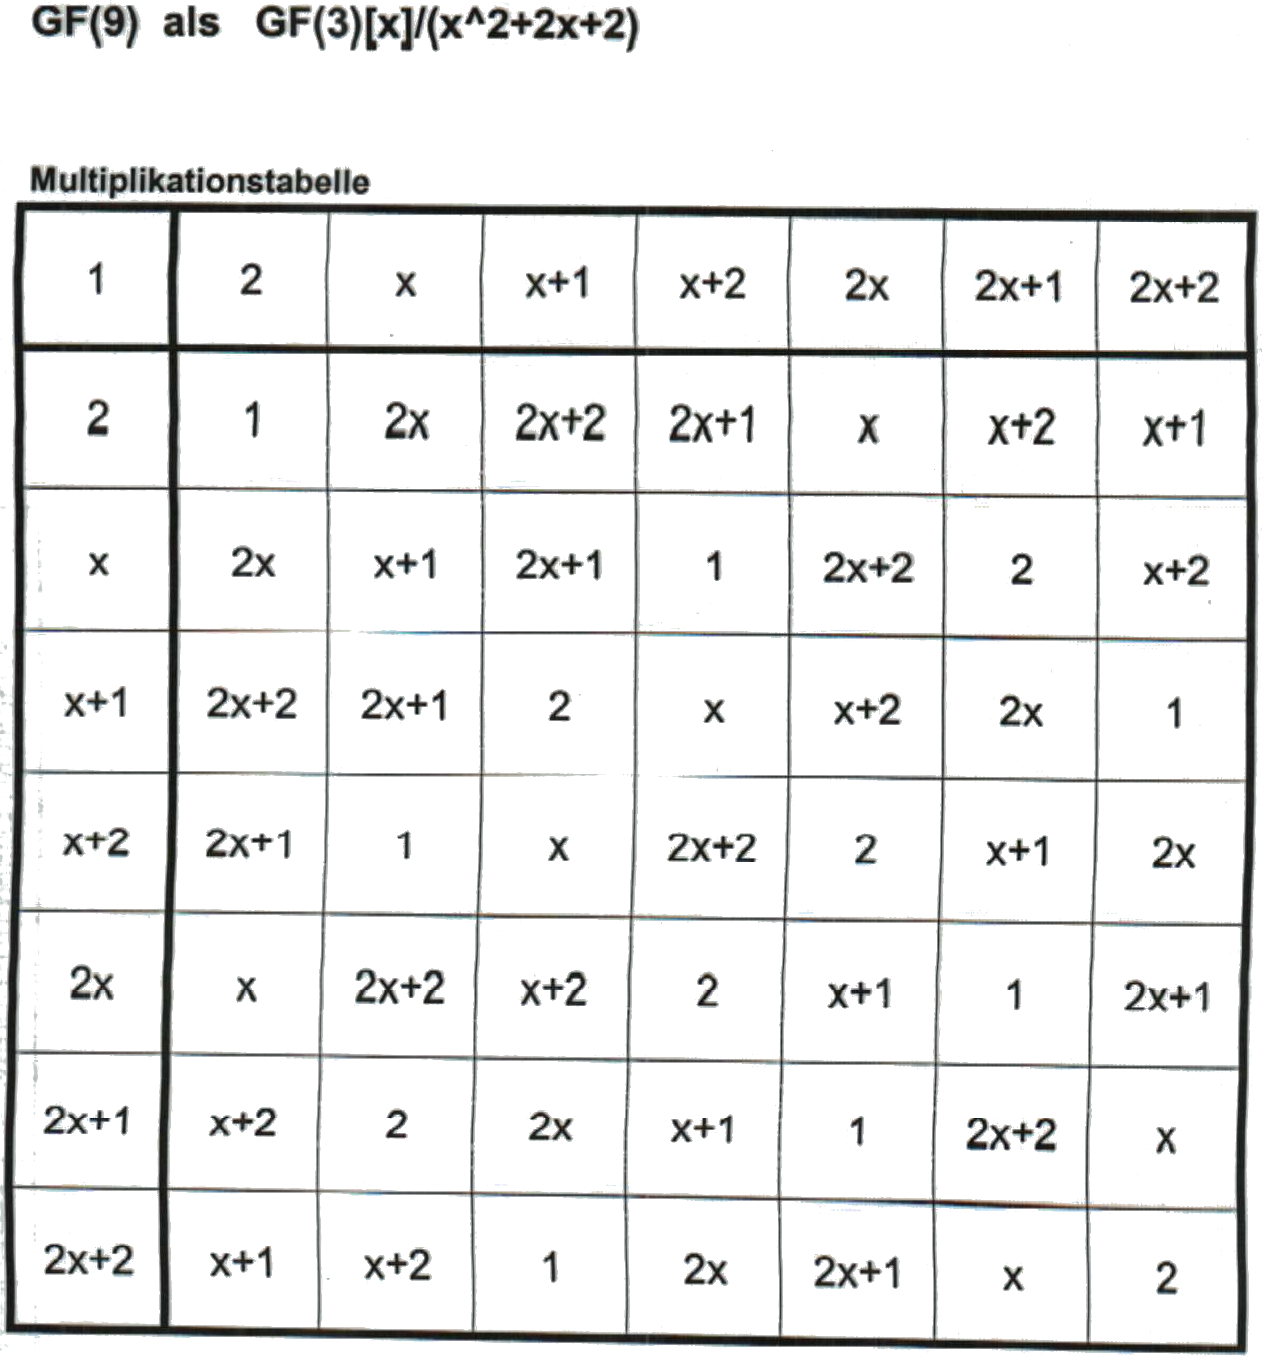
\includegraphics[width=10cm, height=10cm]{mainmatter/chapter3/pics/multitabelle.png}
\caption{Eine Multiplikationstabelle} 
\end{figure}
 
	 
	\backmatter 
		\listoffigures 
\end {document}
